\documentclass{article}
\usepackage[utf8]{inputenc}
\usepackage{graphicx}
\usepackage{caption}
\usepackage{algorithm}
\usepackage{algorithmic}
\usepackage[linesnumbered,ruled,vlined]{algorithm2e}
\usepackage{amsmath, amssymb} 

\usepackage{graphicx}
\usepackage{subcaption}
\usepackage{hyperref}
% per utilizzare l'ambiente equation e comandi matematici
\usepackage{datetime} % se stai manipolando oggetti di tipo datetime
\usepackage[hidelinks]{hyperref} % Disabilita i contorni dei collegamenti

\newcommand{\Rel}[1]{\mathsf{#1}}


% Adjust indentation (left indent, right indent)
\SetInd{0.15em}{0.15em}
\usepackage[english]{babel}

\RequirePackage{tikz}
% !TeX root = main.tex

\usepackage{graphicx}


\usepackage{tikz}
\usetikzlibrary{arrows,shapes}
\usetikzlibrary{arrows.meta}
\usetikzlibrary{calc}
\usetikzlibrary{math}

\colorlet{MyGreen}{green!50!black}


%%%%%%%%%%%%%%%%%%%%%%%%%%%%%%%% RELATION PLOTS %%%%%%%%%%%%%%%%%%%%%%%%%%%%%%%%



\pgfdeclarelayer{shading}
\pgfdeclarelayer{grid}
\pgfdeclarelayer{overlay}
\pgfdeclarelayer{axes}
\pgfdeclarelayer{tuples}
\pgfsetlayers{shading,grid,overlay,tuples,axes,main}


\tikzstyle{relations}       = [yscale = 0.4]
\tikzstyle{axis}            = []  
%\tikzstyle{axis}            = [x=.3cm, y=.3cm]     % changed
\tikzstyle{axis label}      = [font = \scriptsize, inner sep = 0, outer sep = 3pt]
\tikzstyle{x axis label}    = [axis label, anchor = 110]
\tikzstyle{y axis label}    = [axis label, anchor = -20]
\tikzstyle{axis tick}       = [thin]
\tikzstyle{axis tick label} = [font = {\normalfont\scriptsize}, inner sep = 0, outer sep = 4pt]
\tikzstyle{grid}            = [thin, lightgray] 
%\tikzstyle{grid}            = [thin, lightgray, x=.3cm, y=.3cm]  % changed
\tikzstyle{tuple}           = [line width = 1mm]
\tikzstyle{old tuple}       = [tuple, gray, dash pattern = on 1mm off 1mm]
\tikzstyle{tuple label}     = [font = \small, at start, anchor = south west,
    inner ysep = 1.5pt, inner xsep = 1pt]
\tikzstyle{overlay line}    = [orange, line width = 2mm]


\newcommand*{\DrawXAxis}[3] % width, height, separator elevation
{
    \pgfmathsetmacro{\MaxX}{#1}
    \pgfmathsetmacro{\MaxY}{#2}

    \begin{pgfonlayer}{grid}
        \ifnum#3>0
        \draw [grid] (0, #3) -- (\MaxX, #3);
        \fi
        \foreach \x in {0, ..., \MaxX}
        \draw [grid] (\x, 0) -- +(0, \MaxY);
    \end{pgfonlayer}

    \begin{pgfonlayer}{axes}
        \draw[axis, ->] (0, 0) -- (\MaxX, 0) node [x axis label] {$t$};
        \pgfmathparse{\MaxX - 1}
        \foreach \x in {0, ..., \pgfmathresult}
        {
        \draw[axis tick] (\x, -0.2) -- (\x, 0.2);
        \node[axis tick label, anchor = north] at (\x, 0) {\x};
        }
    \end{pgfonlayer}
}




\newcommand*{\DrawAxes}[2] % width, height
{
\pgfmathsetmacro{\MaxX}{#1}
\pgfmathsetmacro{\MaxY}{#2}

\DrawXAxis{\MaxX}{\MaxY}{0}

\begin{pgfonlayer}{grid}
    \foreach \y in {1, ..., \MaxY}
    \draw [grid] (0, \y) -- +(\MaxX, 0);
\end{pgfonlayer}

\begin{pgfonlayer}{axes}
    \draw[axis, ->] (0, 0) -- (0, \MaxY) node [y axis label] {$A$} ;
    \pgfmathparse{\MaxY - 1}
    \foreach \y in {0, ..., \pgfmathresult}
    {
    \draw[axis tick] (-0.1, \y) -- (0.1, \y);
    \node[axis tick label, anchor = east] at (0, \y) {\y};
    }
\end{pgfonlayer}
}




\newcommand*{\DrawTuple}[5][tuple] % [style,] start, end, elevalion, name
{
    \begin{pgfonlayer}{tuples}
        \draw[#1] (#2, #4) -- (#3, #4) node [tuple label] {#5};
    \end{pgfonlayer}
}



\newcommand*{\DrawRTuple}{}
\newcommand*{\ResetDrawRTuple}{
    \renewcommand*{\DrawRTuple}[4]{\DrawTuple{##1}{##2}{##3}{##4}}
}
\ResetDrawRTuple



\newcommand*{\DrawISEQLExampleRelations}
{
    \DrawXAxis{8}{7}{3}

    \DrawRTuple{0}{1}{5}{$r_1$}
    \DrawRTuple{1}{3}{6}{$r_2$}
    \DrawRTuple{2}{5}{4}{$r_3$}

    \DrawTuple{1}{3}{2}{$s_1$}
    \DrawTuple{3}{4}{1}{$s_2$}
}


%%%%%%%%%%%%%%%%%%%%%%%%%%%%%%%%%%%% DOODLES %%%%%%%%%%%%%%%%%%%%%%%%%%%%%%%%%%%


\newsavebox{\IgnoreBox}
\tikzset
{
    ignore/.style = % https://tex.stackexchange.com/questions/232588
    {
        draw = none,
        fill = none,
        overlay,
        execute at begin node = {\begin{lrbox}{\IgnoreBox}},
        execute at end node = {\end{lrbox}}
    },
    table interval algebra relation/.style =
    {
        xscale = 0.5,
        yscale = 0.2,
        interval/.style = {line width = 1pt, > = {Circle[length = 3.4pt]},
            shorten > = -0pt},
        baseline = {($(current bounding box.north) - (0,7.5pt)$)},
        interval label/.style = {font = {\small}},
        vertical separator/.style = {very thin, overlay},
    },
    inline interval algebra relation/.style =
    {
        xscale = 0.1,
        yscale = 0.1,
        baseline = -1pt,
        interval/.style = {line width = 0.5pt, > = {Circle[length = 1.4pt]},
            shorten > = 0pt},
        interval label/.style = {ignore},
        vertical separator/.style = {ignore},
    },
}


\newcommand*{\Doodle}[2][inline] % [style], content
{%
    \begin{tikzpicture}[#1 interval algebra relation]
        #2
    \end{tikzpicture}%
}


\newcommand*{\Interval}[5][] % [style], start, end, elevation, name
{
    \draw[interval, #1] (#2, #4) -- (#3, #4);
    \node[interval label] at (-0.5,#4) {#5};
}


\newcommand*{\RSIntervals}[6] % r style, r start, r end, s style, s start, s end
{
    \Interval[#1]{#2}{#3}{1}{$r$}
    \Interval[#4]{#5}{#6}{0}{$s$}
}


\newcommand*{\Reverse}[1]
{
    \begin{scope}[yscale = -1, yshift = -1cm]
      #1
    \end{scope}
}


\newcommand*{\LeftOverlap}
{
    \RSIntervals
        {<->}{0}   {2}
        {<->}   {1}   {3}
}

\newcommand*{\During}
{
    \RSIntervals
        {<->}   {1}{2}
        {<->}{0}      {3}
}

\newcommand*{\StartPreceding}
{
    \RSIntervals
        {<- }{0}      {3}
        {<- }   {1}   {3}
}

\newcommand*{\EndFollowing}
{
    \RSIntervals
        { ->}{0}      {3}
        { ->}{0}   {2}
}

\newcommand*{\Before}
{
    \RSIntervals
        { ->}{0}{1}
        {<- }      {2}{3}
}


\newcommand*{\Meets}
{
    \RSIntervals
        { ->}{0}{1.495}
        {<- }        {1.505}{3}
    \draw [vertical separator] (1.5, -0.5) -- (1.5, 1.5);
}


\newcommand*{\Starts}
{
    \RSIntervals
        {<->}{0}{1.5}
        {<->}{0}     {3}
}





\newcommand*{\Finishes}
{
    \RSIntervals
        {<->}   {1.5}{3}
        {<->}{0}     {3}
}



\newcommand*{\Equals}
{
    \RSIntervals
        {<->}{0}     {3}
        {<->}{0}     {3}
}


\newcommand*{\Overlaps}{\LeftOverlap}



%%%%%%%%%%%%%%%%%%%%%%%%%%%%%%%%%%%%%%%% changed (added)


\newcommand*{\DrawXAxisNarrow}[3] % width, height, separator elevation     (changed)
{
    \pgfmathsetmacro{\MaxX}{#1}
    \pgfmathsetmacro{\MaxY}{#2}

    \begin{pgfonlayer}{grid}
        \ifnum#3>0
        \draw [grid] (0, #3) -- (\MaxX/2, #3);
        \fi
        \foreach \x in {0, ..., \MaxX}
        \draw [grid] (\x/2, 0) -- +(0, \MaxY);
    \end{pgfonlayer}

    \begin{pgfonlayer}{axes}
       \draw[axis, ->] (0, 0) -- (\MaxX/2, 0) node [x axis label] {$t$};
        \pgfmathparse{\MaxX - 1}
        \foreach \x in {0, ..., \pgfmathresult}
        {
        \draw[axis tick] (\x/2, -0.2) -- (\x/2, 0.2);
        \node[axis tick label, anchor = north] at (\x/2, 0) {\x};
        }
    \end{pgfonlayer}
}


\newcommand*{\DrawXAxisNarrowTwoSep}[4] % width, height, 2 separator elevation (changed)
{
    \pgfmathsetmacro{\MaxX}{#1}
    \pgfmathsetmacro{\MaxY}{#2}

    \begin{pgfonlayer}{grid}
        \ifnum#3>0
        \draw [grid] (0, #3) -- (\MaxX/2, #3);
        \fi
        \foreach \x in {0, ..., \MaxX}
        \draw [grid] (\x/2, 0) -- +(0, \MaxY);
    \end{pgfonlayer}

    \begin{pgfonlayer}{grid}
        \ifnum#4>0
        \draw [grid] (0, #4) -- (\MaxX/2, #4);
        \fi
        \foreach \x in {0, ..., \MaxX}
        \draw [grid] (\x/2, 0) -- +(0, \MaxY);
    \end{pgfonlayer}

    \begin{pgfonlayer}{axes}
       \draw[axis, ->] (0, 0) -- (\MaxX/2, 0) node [x axis label] {$t$};
        \pgfmathparse{\MaxX - 1}
        \foreach \x in {0, ..., \pgfmathresult}
        {
        \draw[axis tick] (\x/2, -0.2) -- (\x/2, 0.2);
        \node[axis tick label, anchor = north] at (\x/2, 0) {\x};
        }
    \end{pgfonlayer}
}


\newcommand*{\DrawTupleNarrow}[5][tuple] % [style,] start, end, elevation, name
{
    \begin{pgfonlayer}{tuples}
        \draw[#1] (#2/2, #4) -- (#3/2, #4) node [tuple label] {#5};
    \end{pgfonlayer}
}



\newcommand*{\DrawPointA}[5][tuple] % [style,] start, end, elevation, name
{
    \begin{pgfonlayer}{tuples}
        \fill[#1,brown] (#2/2,#4) ellipse (2pt and 10pt) node[left] {#5};
    \end{pgfonlayer}
}


\newcommand*{\DrawPointB}[5][tuple] % [style,] start, end, elevation, name
{
    \begin{pgfonlayer}{tuples}
        \fill[purple] (#2/2,#4) ellipse (4pt and 4.5pt) node[left] {#5};
    \end{pgfonlayer}
}


\newcommand*{\DrawText}[5][tuple] % [style,] start, end, elevation, name
{
    \begin{pgfonlayer}{tuples}
        \draw[black] (#2/2,#4) node[right] {#5};
    \end{pgfonlayer}
}


\newcommand*{\DrawTupleA}[5][tuple] % [style,] start, end, elevation, name
{
    \begin{pgfonlayer}{tuples}
        \draw[#1] (#2/2, #4) -- (#3/2, #4) node [tuple label] {#5};
         \tikzmath {
           \z = #2 + 1;
        }       
        \draw[ultra thick,-{Diamond[]}] (#3/2, #4) -- (#2/2-.2, #4);
        \foreach \x in {\z, ..., #3}
        \draw[ultra thick,-{Diamond[]}] (\x/2, #4) -- (\x/2+.2, #4);
    \end{pgfonlayer}
}


\newcommand*{\DrawTupleB}[5][tuple] % [style,] start, end, elevation, name
{
    \begin{pgfonlayer}{tuples}
        \draw[#1,red] (#2/2, #4) -- (#3/2, #4) node [tuple label] {#5};
        \tikzmath {
           \z = #2 + 1;
        }
        \draw[ultra thick,-{Turned Square[]},red] (#3/2, #4) -- (#2/2-.165, #4);
        \foreach \x in {\z, ..., #3}
          \draw[ultra thick,-{Turned Square[]},red] (\x/2, #4) -- (\x/2+.165, #4);
    \end{pgfonlayer}
}




\newcommand*{\DrawTupleC}[5][tuple] % [style,] start, end, elevation, name
{
    \begin{pgfonlayer}{tuples}
        \draw[#1,blue] (#2/2, #4) -- (#3/2, #4) node [tuple label] {#5};
        \tikzmath {
           \z = #2 + 1;
        }
        \draw[ultra thick,-{Circle[]},blue] (#3/2, #4) -- (#2/2-.14, #4);
        \foreach \x in {\z, ..., #3}
          \draw[ultra thick,-{Circle[]},blue] (\x/2, #4) -- (\x/2+.14, #4);
    \end{pgfonlayer}
}


\newcommand*{\DrawTupleD}[5][tuple] % [style,] start, end, elevation, name
{
    \begin{pgfonlayer}{tuples}
        \draw[#1,orange] (#2/2, #4) -- (#3/2, #4) node [tuple label] {#5};
        \tikzmath {
           \z = #2 + 1;
        }
        \draw[ultra thick,-{Square[]},orange] (#3/2, #4) -- (#2/2-.13, #4);
        \foreach \x in {\z, ..., #3}
          \draw[ultra thick,-{Square[]},orange] (\x/2, #4) -- (\x/2+.13, #4);
    \end{pgfonlayer}
}


\newcommand*{\DrawTupleE}[5][tuple] % [style,] start, end, elevation, name
{
    \begin{pgfonlayer}{tuples}
        \draw[#1,gray] (#2/2, #4) -- (#3/2, #4) node [tuple label] {#5};
        \tikzmath {
           \z = #2 + 1;
        }
        \draw[ultra thick,-{Tee Barb[]},gray] (#3/2, #4) -- (#2/2-.09, #4);
        \foreach \x in {\z, ..., #3}
          \draw[ultra thick,-{Tee Barb[]},gray] (\x/2, #4) -- (\x/2+.09, #4);
    \end{pgfonlayer}
}


\newcommand*{\DrawTupleF}[5][tuple] % [style,] start, end, elevation, name
{
    \begin{pgfonlayer}{tuples}
        \draw[#1,green] (#2/2, #4) -- (#3/2, #4) node [tuple label] {#5};
        \tikzmath {
           \z = #2 + 1;
        }
        \draw[ultra thick,-{Rays[]},green] (#3/2, #4) -- (#2/2-.14, #4);
        \foreach \x in {\z, ..., #3}
          \draw[ultra thick,-{Rays[]},green] (\x/2, #4) -- (\x/2+.14, #4);
    \end{pgfonlayer}
}


\newcommand*{\DrawTupleG}[5][tuple] % [style,] start, end, elevation, name
{
    \begin{pgfonlayer}{tuples}
        \draw[#1,olive] (#2/2, #4) -- (#3/2, #4) node [tuple label] {#5};
        \tikzmath {
           \z = #2 + 1;
        }
        \draw[ultra thick,-{Rays[n=9]},olive] (#3/2, #4) -- (#2/2-.14, #4);
        \foreach \x in {\z, ..., #3}
          \draw[ultra thick,-{Rays[n=9]},olive] (\x/2, #4) -- (\x/2+.14, #4);
    \end{pgfonlayer}
}

\newcommand*{\DrawTupleH}[5][tuple] % [style,] start, end, elevation, name
{
    \begin{pgfonlayer}{tuples}
        \draw[#1,magenta] (#2/2, #4) -- (#3/2, #4) node [tuple label] {#5};
        \tikzmath {
           \z = #2 + 1;
        }
        \draw[ultra thick,-{Circle[open]},magenta] (#3/2, #4) -- (#2/2-.14, #4);
        \foreach \x in {\z, ..., #3}
          \draw[ultra thick,-{Circle[open]},magenta] (\x/2, #4) -- (\x/2+.14, #4);
    \end{pgfonlayer}
}

\newcommand*{\DrawTupleI}[5][tuple] % [stile,] inizio, fine, elevazione, nome
{
    \begin{pgfonlayer}{tuples}
        \draw[#1,red!80!black] (#2/2, #4) -- (#3/2, #4) node [tuple label] {#5};
        \tikzmath {
           \z = #2 + 1;
        }
        \draw[ultra thick,-{Turned Square[]},red!80!black] (#3/2, #4) -- (#2/2-.165, #4);
        \foreach \x in {\z, ..., #3}
          \draw[ultra thick,-{Turned Square[]},red!80!black] (\x/2, #4) -- (\x/2+.165, #4);
    \end{pgfonlayer}
}

\newcommand*{\DrawTupleJ}[5][tuple] % [stile,] inizio, fine, elevazione, nome
{
    \begin{pgfonlayer}{tuples}
        \draw[#1,blue!30] (#2/2, #4) -- (#3/2, #4) node [tuple label] {#5};
        \tikzmath {
           \z = #2 + 1;
        }
        \draw[ultra thick,-{Circle[]},blue!30] (#3/2, #4) -- (#2/2-.14, #4);
        \foreach \x in {\z, ..., #3}
          \draw[ultra thick,-{Circle[]},blue!30] (\x/2, #4) -- (\x/2+.14, #4);
    \end{pgfonlayer}
}



% \newcommand*{\DrawSpammingA}
% {
%     \DrawXAxisNarrow{16}{4}{0}
%
%     \DrawTupleD{1}{15}{3}{session}
%     \DrawPointA{1}{1}{2}{login}
%     \DrawTupleC{2}{14}{1}{sharing}
%     \DrawPointB{15}{15}{2}{logout}
% }


\newcommand*{\DrawSpammingTS}   
{
    \DrawXAxisNarrow{8}{5}{0}
    
    \DrawTupleB{2}{4}{4.5}{high}
    \DrawTupleD{4}{5}{3}{normal}
    \DrawTupleC{5}{6}{1}{low}
}

\newcommand*{\DrawSpammingAD}   
{
    \DrawXAxisNarrow{8}{4}{0}
    
    \DrawTupleB{2}{6}{2}{high}

}

\newcommand*{\DrawSpammingAF}   
{
    \DrawXAxisNarrow{8}{4}{0}
    
    \DrawTupleC{1}{2}{2}{low}
    \DrawTupleC{3}{4}{2}{low}
    \DrawTupleC{5}{6}{2}{low}

}

\newcommand*{\DrawSpammingTSAD}   
{
    \DrawXAxisNarrow{8}{5}{0}

    \DrawTupleC{1}{2}{1}{low}
    \DrawTupleD{2}{3}{3}{normal}
    \DrawTupleB{3}{6}{4.5}{high}
   
}

\newcommand*{\DrawSpammingEHAD}   
{
    \DrawXAxisNarrow{8}{5}{0}

    \DrawTupleI{3}{5}{3}{extremely high}
   
}

\newcommand*{\DrawSpammingELAF}   
{
    \DrawXAxisNarrow{8}{5}{0}

    \DrawTupleJ{2}{3}{3}{extremely low}
    \DrawTupleJ{4}{5}{3}{}
    \DrawTupleJ{6}{7}{3}{}


   
}

\newcommand*{\DrawSpammingTSAF}   
{
    \DrawXAxisNarrow{9}{5}{0}

    \DrawTupleB{0}{1}{4.5}{high}
    \DrawTupleD{1}{2}{3}{normal}
    \DrawTupleC{2}{3}{1}{low}
    \DrawTupleD{3}{4}{3}{normal}
    \DrawTupleB{4}{6}{4.5}{high}
    \DrawTupleD{6}{7}{3}{normal}
    \DrawTupleC{7}{8}{1}{low}




   
}
    


% \newcommand*{\DrawSpammingB}
% {
%     \DrawXAxisNarrow{16}{5}{0}
%
%     \DrawTupleD{1}{15}{4}{session}
%     \DrawPointA{1}{1}{3}{login}
%     \DrawTupleC{2}{3}{2}{sharing}
%     \DrawTupleA{4}{5}{1}{liking}
%     \DrawTupleB{6}{8}{2}{sharing}
%     \DrawTupleE{9}{10}{1}{liking}
%     \DrawTupleF{11}{14}{2}{sharing}
%     \DrawPointB{15}{15}{1}{logout}
% }



% \newcommand*{\DrawFragileAllen}
% {
%     \DrawXAxisNarrowTwoSep{16}{9}{6}{3}
%
%     \DrawTupleC{3}{5}{8}{posting}
%     \DrawTupleB{5}{9}{7}{sending}
%     \DrawText{12}{12}{8}{\JoinName{meets}}
%
%     \DrawTupleC{3}{5}{5}{posting}
%     \DrawTupleB{7}{10}{4}{sending}
%     \DrawText{12}{12}{5}{\JoinName{before}}
%
%     \DrawTupleC{3}{5}{2}{posting}
%     \DrawTupleB{4}{7}{0.5}{sending}
%     \DrawText{12}{12}{2}{\JoinName{overlap}}
% }





%%%%%%%%%%%%%%%%%%%%%%%%%%%%%%%%%%%%%%%%%%%%%%%%%%%%%%%%%%%%%%%%%%%%%%%%%%%%%%

\newcommand*{\DrawIntervalTimestampJoinStart}    % just here for testing purposes
{
    \DrawXAxisNarrow{16}{7}{4}
    
    \DrawTupleNarrow[red,line width=1mm]{0}{ 5}{6}{$r_1$}
    \DrawTupleNarrow[blue,line width=1mm]{0}{10}{5}{$r_2$}
    \DrawTupleNarrow[black,line width=1mm]{6}{11}{6}{$r_3$}
    
    \DrawTupleA{1}{ 2}{2}{$s_1$}
    \DrawTupleB{2}{12}{1}{$s_2$}
    \DrawTupleC{3}{ 5}{2}{$s_3$}
    \DrawTupleD{10}{ 14}{2}{$s_6$}    
    \DrawPointA{4}{4}{3}{$s_4$}
    \DrawPointB{9}{ 9}{3}{$s_5$}
}




\title{ISEQL-Glucose Analyzer}
\author{Lorenzo Tucceri Cimini}
\date{\today}

\begin{document}

\maketitle

\begin{abstract}

Managing diabetes requires continuous monitoring of blood glucose levels to prevent complications. This project focuses on analyzing time-series glucose data to model different glycemic conditions: normal, extremely high, high, low, and extremely low. Using Python tools like Pandas and NumPy, we perform data cleaning, segmentation into intervals, and employ ISEQL for complex event detection. Our proposed architecture includes a Data Crawler for raw data extraction, an Interval Action Detector for event annotation, and a High-Level Event Detector for complex event identification. Results highlight effective glucose level analysis for diabetes management, emphasizing pattern recognition and anomaly detection across various time intervals. This approach enhances understanding of glucose behaviors critical for personalized treatment strategies.

\end{abstract}


\section{Introduction}

Continuous monitoring of blood glucose is essential for managing diabetes, a chronic condition that necessitates precise control of blood sugar levels to prevent complications. This project focuses on analyzing a dataset of glucose values recorded over time, with the aim of identifying and modeling time intervals associated with different glycemic conditions: \textbf{normal}, \textbf{high}, \textbf{extremely high}, \textbf{low}, and \textbf{extremely low}.

Utilizing data analysis tools in Python, such as Pandas for data manipulation and NumPy for numerical operations, we will extract meaningful insights from the raw data. Additionally, we will employ ISEQL (\textbf{Interval-based Surveillance Event Query Language}) to formally define and detect complex events in health data. ISEQL is particularly suitable for this analysis as it allows for the combination of low-level events into more sophisticated structures, enhancing the expressiveness and efficiency of the event detection process.

The analysis will proceed with data cleaning and preparation, followed by segmentation into relevant time intervals. We will then use ISEQL to define and detect complex events, concluding with a discussion of the results and their implications for diabetes management.

We will work with a CSV file containing glucose data from the past 90 days, specifically from February 13, 2024, to May 12, 2024. Our analysis will focus on:

\begin{itemize}
    \item \textbf{Simple High-Level Event}:
        \begin{itemize}
            \item \textbf{Time Swing}: Identifying individual glycemic events and significant changes in glucose levels, highlighting rapid fluctuations between different glucose categories.
            \item \textbf{Too Long Glucose Anomalies}: Measuring the time spent in anomalous glucose ranges, which may indicate deteriorating health conditions.
        \end{itemize}
    \item \textbf{Aggregated High-Level Event}: Aggregating multiple events to provide a comprehensive view of glucose level anomalies. This includes:
    \begin{itemize}
        \item \textbf{Too Frequent Glucose Anomalies}: Assessing the frequency of anomalous glucose events within the observation period.
        \item \textbf{Too Frequent Time Swings}: Evaluating the frequency of rapid glucose level changes within a specific time frame, indicating potential issues with glucose stability.
        \item \textbf{Time Swing With Too Long Glucose Anomalies}: Analyzing swings where one of the intervals before or after the swing has a Too Long Glucose Anomalies, indicating extended instability.
    \end{itemize}
\end{itemize}

These methods will help us identify significant correlations and trends in the data, which are crucial for effective diabetes management. By distinguishing between simple and aggregated high-level events, we can better understand and respond to complex glucose level patterns, ultimately improving patient care and outcomes.


\section{State of Art}

Diabetes represents a global health challenge, with artificial intelligence (AI) revolutionizing disease management. AI, leveraging its ability to analyze vast amounts of data and identify complex patterns, promises significant improvements in diagnosis, personalized treatment, and diabetes management. In this section, we will explore various tools used for studying and analyzing this disease, including advanced monitoring devices like the Dexcom G7, which provide essential data to optimize daily diabetes management.


\begin{itemize}
    \item Dexcom G7
    \item DiaHealth
    \item Blood Glucose Level Prediction with Feedforward Neural Network
\end{itemize}

\subsection{Dexcom G7}

The Dexcom G7 represents one of the latest advancements in CGM technology, distinguished by its effectiveness and convenience. The device provides glucose level updates every 5 minutes, enabling users to closely monitor glycemic fluctuations throughout the day. A detailed graph displays glucose trends over the past 24 hours, facilitating the identification of significant glycemic peaks and valleys through customizable thresholds.

Additionally, Dexcom Clarity offers a long-term overview of glucose trends, allowing users to analyze data from the past 90 days through detailed charts and statistics on glycemic quality. This feature supports not only informed daily management but also preventive strategies to reduce the risk of long-term diabetes complications.

In-depth studies have shown that accurate and continuous glucose monitoring can lead to significant improvements in health management by early identification of issues such as prolonged periods of hyperglycemia or rapid shifts between hypoglycemia and hyperglycemia.

In our case, we use data about glucose provided by Dexcom.

\subsection{DiaHealth}

DiaHealth is an innovative mobile application designed to enhance daily diabetes management through a comprehensive range of integrated features. This application stands out in the landscape of digital diabetes solutions by integrating artificial intelligence to offer personalized suggestions and support more effective disease management.

Key features of DiaHealth include:

\begin{itemize}
    \item \textbf{Blood Glucose Monitoring}: Allows users to regularly monitor their blood glucose levels through an intuitive and user-friendly interface.
    
    \item \textbf{Diet and Exercise Plans}: Provides personalized plans for diet and physical activity, helping users maintain a healthy and balanced lifestyle.
    
    \item \textbf{Health Data Logging}: Enables users to record and monitor various health parameters such as blood glucose, blood pressure, HbA1c, cholesterol, and weight.
    
    \item \textbf{Smart Suggestions}: Uses artificial intelligence to analyze user-entered data and provide personalized suggestions to improve diabetes control.
    
    \item \textbf{Diabetes Education}: Offers educational resources to help users better understand their condition and adopt healthy behaviors.
\end{itemize}

In our context, it is an excellent starting point to leverage High-Level Events and provide suggestions on glucose management, physical activity, and diet.

\subsection{Blood Glucose Level Prediction with Feedforward Neural Network}

Feedforward neural networks (FNNs) are applied for predicting blood glucose levels using historical data from continuous monitoring systems (CGM) such as Dexcom G7. These models are designed to process sequences of past glucose measurements. The architecture of an FNN includes an input layer for previous measurements, hidden layers that extract features and learn temporal dependencies, and an output layer that predicts future glucose levels over a specific time interval, such as 15 minutes.

FNNs have demonstrated high accuracy in predicting glucose levels, as evidenced by low Root Mean Square Error (RMSE) values. This indicates the model's ability to effectively manage individual variations in diabetes management factors such as insulin sensitivity, meal timing, and physical activity levels. Thanks to these precise predictions, FNNs enable proactive management of glucose fluctuations, significantly reducing the incidence of hyperglycemic and hypoglycemic episodes.

This study could provide a deeper understanding of high-level events by predicting glucose levels and the possible events that follow.



\section{Overview and Formalization}

The overall architecture of the glucose level monitoring system we propose is shown in Figure 1. It consists of three levels: a \textit{Data Crawler}, an \textit{Interval Action Detector}, and a \textit{High-Level Event Detector}.

The \textit{Data Crawler} extracts data from a continuous glucose monitoring sensor, specifically the Dexcom. This sensor releases a dataset with blood glucose level measurements every 5 minutes. The raw events thus correspond to these periodic glucose level measurements. Consequently, this level is highly dependent on the application domain and allows us to obtain data with specific timestamps. Clearly, the \textit{Data Crawler} must include all the necessary components to extract and process this timestamped data, such as a library to collect and manage data from the Dexcom.

In the next step, the \textit{Interval Action Detector} takes the raw events and creates simple events whose format is largely independent of the application domain. This separates the High-Level Event Detection from the technical details of the raw events. As a result, this level produces a set M of mid-level annotations referring to intervals of glucose level readings, with timestamps, corresponding to the mid-level predicates Pr stored in the knowledge base (Figure 4). Additionally, the events generated by this level already contain some aggregated data, thus simplifying High-Level Event Detection.

Finally, at the highest level, a user can construct complex events of real interest using mid-level events and simpler high-level events as building blocks. We also provide a graphical user interface to formulate high-level events. Consequently, the \textit{High-Level Event Detector} takes a set E of event patterns and determines if any of these events occur in M.

In summary, compared to the approaches listed in Section 2, ours presents the following advantages:

\begin{itemize}
    \item Generalizable to heterogeneous domains (Figure 1);
    \item Flexible in defining new event patterns, thanks to the robust support of an intelligent graphical user interface (Figure 1);
    \item Adaptable whenever a new low-level event representing a new glucose level pattern is detected by the \textit{Data Crawler}; it is immediately and easily mapped to higher levels, and thus exploitable for defining new event patterns;
    \item Effective and efficient in detecting the occurrences of events of interest;
    \item Combinable with machine learning approaches; we could learn event patterns through machine learning approaches, then easily define and detect their occurrences;
    \item Significantly improves glucose level analysis;

    \item In addition to the aforementioned advantages, our system introduces novel high-level event types that are not commonly available in other applications. For example, we have defined events like "Time Swing" and its variants, which identify specific patterns in glucose level fluctuations over time. These new high-level events offer a more nuanced understanding of glucose level behavior, enhancing the monitoring and management of blood glucose levels. The inclusion of these unique event patterns significantly broadens the analytical capabilities of our system.
\end{itemize}

\begin{figure}[h]
    \centering
    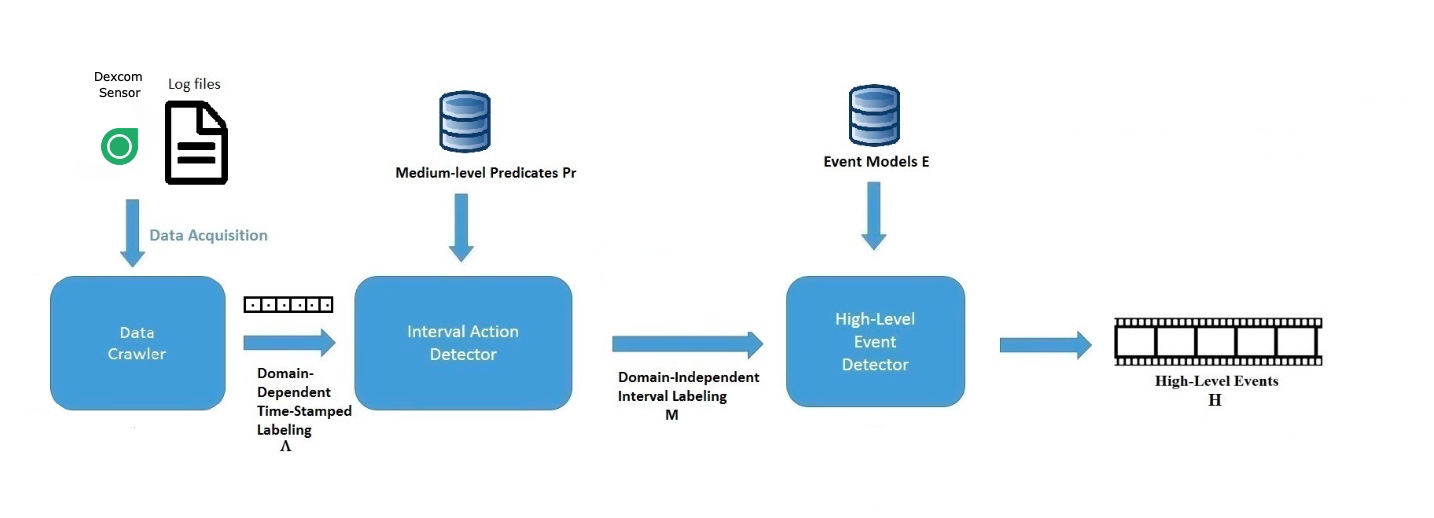
\includegraphics[width=1.0\textwidth]{Images/architecture.png}
    \caption{Overall Architecture}
    \label{fig:architecture}
\end{figure}

\subsection{Data Crawler}

To better understand various glucose level events, we use symbolic notation to represent each type of event and its corresponding thresholds. The following table shows the correspondence between symbols, events, and thresholds (i.e., the glucose level domain):


\begin{table}[h!]
    \centering
    \begin{tabular}{|c|c|c|}
        \hline
        \textbf{Symbol} & \textbf{Event} & \textbf{Threshold} \\
        \hline
        a & Extremely High & $\geq$ 250 \\
        b & High & $ 180 \leq  x < 250$ \\
        c & Normal & $80 < x < 180$ \\
        d & Low & $55 < x \leq 80$ \\
        e & Extremely Low & $\leq$ 55 \\
        \hline
    \end{tabular}
    \caption{Mapping of Events and Thresholds with Symbols (S))}
    \label{tab:events}
\end{table}

The Data Crawler will associate events in Table \ref{tab:events} with glucose levels extracted from the dataset. Here we introduce the first definition.\\

\textbf{Definition 1 (Timestamp Labeling of Glucose Level).} In the domain of glucose levels, timestamp labeling is a tuple \(\lambda = (s, ts, gl)\), where \(\lambda.s \in S\) (Table \ref{tab:events}) represents the state associated with the event, \(\lambda.ts\) is the timestamp related to the event state, and \(\lambda.gl\) represents the glucose level at that specific moment. A timestamp labeling \(\Lambda\) is a finite set of entries with timestamps \(\lambda_i\) ordered by timestamp.

In the second table, we display the result from the Data Crawler, which includes only the columns of interest: "Symbol," "Timestamp," and "Glucose Level." These data represent glucose levels over time, as shown in Table \ref{tab:glucose_levels}.



\begin{table}[h!]
    \centering
    \begin{tabular}{|c|c|c|}
        \hline
       \textbf{Symbol} & \textbf{Timestamp} & \textbf{Glucose Level} \\
        \hline
        c & 2024-02-13T00:16:32 & 120 \\
        c & 2024-02-13T00:21:33 & 123 \\
        b & 2024-02-13T01:31:32 & 205 \\
        b & 2024-02-13T01:36:33 & 202 \\
        c & 2024-02-13T02:05:32 & 160 \\
        \hline
    \end{tabular}
    \caption{Glucose Level Domain}
    \label{tab:glucose_levels}
\end{table}

\subsection{Interval Action Detector}
In this section, we delve into Interval Action Detection, operating at an intermediate level where we work with temporal intervals. After labeling events based on their thresholds, we organize the data into temporal intervals.

To optimize the selection of intervals of interest, we use the Offline Interval Action Detection algorithm. This algorithm is particularly useful for managing and selecting non-overlapping intervals, thus improving the efficiency of temporal analysis. \\

\textbf{Offline Interval Action Detection Algorithm:}
The Offline Interval Action Detection algorithm selects the maximum subset of non-overlapping intervals from a set of temporal intervals based on specific actions or events. It is particularly effective in contexts where it is necessary to identify and analyze events or actions occurring at distinct points in time, avoiding temporal overlaps.

\RestyleAlgo{ruled}
\begin{algorithm}[H]
\SetAlgoLined
\caption{Offline Interval Action Detection}
\KwData{glucose\_data: DataFrame containing data on glucose levels}
\KwIn{extreme\_high\_threshold $\leftarrow$ 250, high\_threshold $\leftarrow$ 180, low\_threshold $\leftarrow$ 80, extreme\_low\_threshold $\leftarrow$ 55}
\KwResult{Time intervals associated with each glucose level represented as a list of tuples.}
\Begin{
    intervals $\leftarrow$ []\;
    
    events $\leftarrow$ []\;
    
    \ForEach{row in glucose\_data} {
        timestamp $\leftarrow$ row['Date and hour (AAAA-MM-GGThh:mm:ss)']\;\\
        glucose\_value $\leftarrow$ row['Glucose level (mg/dL)']\;
        
        \If{glucose\_value == "Basso"} {
            event, symbol $\leftarrow$ 'extreme\_low', 'd'\;
        } 
        \Else{
            glucose\_level $\leftarrow$ int(glucose\_value)\;
            
            \If{glucose\_level $>=$ extreme\_high\_threshold} {
                event, symbol $\leftarrow$ 'extremely\_high', 'a'\;
            } \If{glucose\_level $>=$ high\_threshold} {
                event, symbol $\leftarrow$ 'high', 'b'\;
            } \If{glucose\_level $<=$ extreme\_low\_threshold} {
                event, symbol $\leftarrow$ 'extremely\_low', 'e'\;
            } \If{glucose\_level $<=$ low\_threshold} {
                event, symbol $\leftarrow$ 'low', 'd'\;
            } \Else{
                event, symbol $\leftarrow$ 'normal', 'c'\;
            }
        }
        
        \If{intervals is empty \textbf{or} intervals[-1][3] != event} {
            intervals.append((symbol, timestamp, timestamp, event))\;
        } \Else {
            intervals[-1] $\leftarrow$ (intervals[-1][0], intervals[-1][1], timestamp, intervals[-1][3])\;
        }
        
        events.append((symbol, event, glucose\_level if glucose\_value != "Basso" else "extreme\_low"))\;
    }
    
    \Return{intervals, events}\;
}
\end{algorithm}


\pagebreak

\textbf{Definition 2 (Interval Labeling).} A Medium-Level annotation is a tuple \(\mu = (pred, p, tss, tse)\), where \(\mu.pred \in S\) is the Medium-Level predicate describing a Medium-Level event. Here, \(\mu.p\) specifies the patient associated with the state, \(\mu.tss\) is the timestamp related to the beginning of the event, and \(\mu.tse\) pertains to the end of the event.

The following table illustrates an example of how these events can be mapped into specific time intervals for the patient Lorenzo T. C.:

\begin{table}[h!]
    \centering
    \begin{tabular}{|c|c|c|c|}
        \hline
        \textbf{Pred} & \textbf{Patient} & \textbf{Start Time} & \textbf{End Time} \\
        \hline
        Normal & Lorenzo T. C. & 13/02/2024 00:01:32 & 13/02/2024 10:46:33 \\
        High & Lorenzo T. C. & 13/02/2024 10:51:33 & 13/02/2024 11:06:32 \\
        Normal & Lorenzo T. C. & 13/02/2024 11:11:33 & 13/02/2024 12:11:33 \\
        High & Lorenzo T. C. & 13/02/2024 12:16:33 & 13/02/2024 13:06:33 \\
        Normal & Lorenzo T. C. & 13/02/2024 13:11:33 & 13/02/2024 17:31:33 \\
        High & Lorenzo T. C. & 13/02/2024 17:36:33 & 13/02/2024 19:41:34 \\
        Normal & Lorenzo T. C. & 13/02/2024 19:46:33 & 13/02/2024 20:26:34 \\
        Low & Lorenzo T. C. & 13/02/2024 20:31:34 & 13/02/2024 20:46:34 \\
        Normal & Lorenzo T. C. & 13/02/2024 20:51:33 & 13/02/2024 21:46:34 \\
        Low & Lorenzo T. C. & 13/02/2024 21:51:34 & 13/02/2024 22:16:33 \\
        \hline
    \end{tabular}
    \caption{Temporal Intervals of Events for Lorenzo T. C.}
    \label{tab:intervals}
\end{table}

In addition to time intervals, it is useful to consider the duration of each interval to better analyze the behavior of blood glucose events. To find these data, we simply calculated \(\mu.tse - \mu.tss\), where \(\mu.tse \geq \mu.tss\). An interval labeling \(\mathcal{M}\) is a finite set of Medium-Level annotations \(\mu_i\). Specifically, \(\forall \mu \in \mathcal{M}, \mu.pred \in \mathcal{P}_r, \mu.tss, \mu.tse \in \mathbb{N}, \mu.tss \leq \mu.tse\).

The following table shows the duration of intervals for the patient Lorenzo T. C.:

\begin{table}[h!]
    \centering
    \begin{tabular}{|c|c|c|}
        \hline
        \textbf{Pred} & \textbf{Patient} & \textbf{Duration} \\
        \hline
        Normal & Lorenzo T. C. & 10 hours, 45 minutes, 1 second \\
        High & Lorenzo T. C. & 14 minutes, 59 seconds \\
        Normal & Lorenzo T. C. & 1 hour, 0 minutes, 0 seconds \\
        High & Lorenzo T. C. & 50 minutes, 0 seconds \\
        Normal & Lorenzo T. C. & 4 hours, 20 minutes, 0 seconds \\
        High & Lorenzo T. C. & 2 hours, 5 minutes, 1 second \\
        Normal & Lorenzo T. C. & 40 minutes, 1 second \\
        Low & Lorenzo T. C. & 15 minutes, 0 seconds \\
        Normal & Lorenzo T. C. & 55 minutes, 1 second \\
        Low & Lorenzo T. C. & 24 minutes, 59 seconds \\
        \hline
    \end{tabular}
    \caption{Interval Duration for Lorenzo T. C.}
    \label{tab:durations}
\end{table}

To further analyze daily patterns and trends in blood glucose levels, we have also created Medium-Level events by aggregating data into daily intervals. This new event, referred to as \textit{daily}, covers the period from midnight (00:00) to 11:59 PM of each day. This approach allows us to perform daily analyses of the events and identify any significant changes or trends that may occur from one day to the next. By examining these \textit{daily} intervals, we can gain insights into the patient's glucose control over time and make informed decisions regarding treatment and management strategies.

\subsection{High-Level Event Detection}

In this section, we focus on High-Level Event Detection, concentrating on analyzing time intervals associated with anomalous blood glucose events. We categorize these events into two distinct levels: Simple High-Level Event and Aggregated High-Level Event. The analysis covers a period of 90 days, specifically from February 13, 2024, to May 12, 2024, and considers both high and low glucose events. This analysis is based on the events identified at the medium level, as defined in Definition 2 (Interval Labeling).

\textbf{Definition 3 (High-Level Event Detection):} A high-level event is a tuple \( o = (e, p, tss, tse, arg_1, \ldots, arg_m) \), where \( o.e \in E \) is the name of the detected high-level event, \( o.p \) is the patient, \( o.tss \) and \( o.tse \) are the start and end times defining the event, and \( o.arg_1, \ldots, o.arg_m \) are the predicate arguments. The set of high-level events \( H \) is a finite sequence of high-level events \( o_i \). Specifically, for each \( o \in H \), \( o.e \in E \), \( o.tss, o.tse \in \mathbb{N} \), and \( o.tss \leq o.tse \).

High-Level Event Detection, as i said before, is structured into two distinct levels: \textbf{Simple High-Level Event} and \textbf{Aggregated High-Level Event}.

\subsubsection{Simple High-Level Event}

In the Simple High-Level Event category, we identify individual events based on single occurrences of abnormal glucose levels.

\begin{enumerate}
    \item \textbf{Time Swing:} This refers to a rapid change in blood glucose levels over a short period, such as a transition from hyperglycemia to hypoglycemia or vice versa. A potential \textit{Time Swing} is defined as a change from high to low glucose levels or vice versa. However, to classify this change as a true \textit{Time Swing}, we must verify that the duration of the change falls within a predefined threshold of two hours.
    
    \textbf{Example 1 (High-Level Events Simple - Time Swing):}
    
    o = (\text{time\_swing}, \text{Lorenzo T.C}, \text{2024-04-17 08:00:00}, \text{2024-04-17 08:50:00}, \text{high}, \text{low}, \text{00:50:00})\\
    
    
    In this example, the "Time Swing" event for patient Lorenzo T.C. starts on April 17, 2024, at 08:00:00 (end of the high event) and ends at 08:50:00 (start of the subsequent event) on the same day, with the glucose level changing from high to low in 50 minutes. In this case, it qualifies as a true \textit{Time Swing} since it occurs within the two-hour threshold.
    
    The following table shows several examples of Time Swings.

    \pagebreak
    
    \begin{table}[h!]
        \centering
        \begin{tabular}{|c|c|c|c|}
            \hline
            \textbf{First event} & \textbf{Second event} & \textbf{Duration TS}  & \textbf{Event Time}\\
            \hline
            high & low & 00:50:00 & 2024-04-17 08:00:00-08:50:00 \\
            \hline
            low & high &  02:20:00 & 2024-03-01 11:40:00-14:00:00 \\
            \hline
            high & low & 01:04:59 & 2024-03-06 22:20:23-23:24:59 \\
            \hline
    
        \end{tabular}
        \caption{Time Swings for patient Lorenzo T. C.}
        \label{tab:time_swing}
    \end{table}

  \item \textbf{Too Long Glucose Anomalies:} Measures the total time a patient's glucose events remain outside the normal range, if it exceeds a predefined duration. Prolonged periods of abnormal glucose events may indicate deteriorating health conditions.
    
    \textbf{Example 2 (Aggregated High-Level Events - Too Long Glucose Anomalies):}
    
     o = (\text{too\_long\_glucose\_anomalies}, Lorenzo T.C,    \text{2024-02-20 08:30:00}, \\ \text{2024-02-20 14:25:00}, \text{high}, \text{0 days 05:55:00}).
     
    In this example, the "Too Long Glucose Anomalies" event for patient Lorenzo T.C. Several intervals of Too Long Glucose Anomalies were found, including one with high blood glucose lasting 5 hours and 55 minutes.
    
    The following table shows various examples of Too Long Glucose Anomalies:

    \begin{table}[h!]
        \centering
        \begin{tabular}{|c|c|c|}
            \hline
            \textbf{Event} & \textbf{Too Long Glucose Anomalies} & \textbf{Event Time} \\
            \hline
            low & 0 days 01:14:59 & 2024-02-17 07:45:00-08:59:59 \\ 
            \hline
            high & 0 days 05:55:00 & 2024-02-20 08:30:00-14:25:00 \\
            \hline
            low & 0 days 01:09:59 & 2024-02-25 18:20:00-19:29:59 \\
            \hline
        \end{tabular}
        \caption{Too Long Glucose Anomalies for patient Lorenzo T. C.}
        \label{tab:too_long_glucose_anomalies}
    \end{table}

\end{enumerate}

\subsubsection{Aggregated High-Level Event}

In the Aggregated High-Level Event category, we aggregate data from multiple events to provide a broader view of glucose level anomalies. This level includes:

\begin{enumerate}
  \item \textbf{Too Frequent Glucose Anomalies:} 
    This High-Level Event counts the number of times a patient's glucose events exceed or fall below the normal thresholds within a specified time frame. Frequent anomalies can reveal patterns that require further investigation. For example, analyzing \textit{daily} intervals—covering the period from midnight (00:00) to 11:59 PM each day—can help identify if there are recurring high or low glucose events on a daily basis, highlighting potential issues with glucose management that may need attention.\\
    \pagebreak
    
    \textbf{Example 3 (Aggregated High-Level Events - Too Frequent Glucose Anomalies ):}

     o = (\text{too\_frequent\_glucose\_anomalies}, Lorenzo T.C, \text{2024-02-13 00:00:00}, \\ \text{2024-02-13 11:59:00},
    \text{count\_extremely\_high}, \text{1}, \text{count\_high}, \text{3}, \text{count\_low}, \text{2}, \text{count\_extremely\_low}, \text{0}, \text{total\_count}, \text{6}).\\
    
     In this example, the "Too Frequent Glucose Anomalies" for the patient Lorenzo T.C. is analyzed over a time interval from February 13, 2024, at 00:00:00 to February 13, 2024, at 11:59:00. During this period, 3 episodes of high blood glucose, 1 of extremely high blood and 2 episodes of low blood glucose were found.
    
    In the following table, we show the count of various examples of the Too Frequent Glucose Anomalies .
    
    \begin{table}[h!]
        \centering
        \begin{tabular}{|c|c|c|c|c|c|}
            \hline
            \textbf{Extremely high} &
            \textbf{high} & \textbf{Low} & \textbf{Extremely low} & \textbf{Total count}  \\
            \hline
            1 & 3 & 2 & 0 & 6 \\
            \hline
        \end{tabular}
        \caption{Too frequent Glucose Anomalies for patient Lorenzo T. C.}
        \label{tab:too_frequent_glucose_anomalies}
    \end{table}

    \item \textbf{Too Frequent Time Swings:} 
    This metric evaluates the occurrence of Time Swings—rapid fluctuations in glucose levels—within a specified time period. It measures how frequently these swings happen, which can indicate issues with glucose stability. For instance, analyzing \textit{daily} intervals, from midnight (00:00) to 11:59 PM each day, can help determine if rapid glucose fluctuations are a daily occurrence, potentially signaling a need for more intensive glucose monitoring and management.\\

    
    \textbf{Example 4 (Aggregated High-Level Events - Too Frequent Time Swings)):}

    o = (\text{too\_frequent\_time\_swings}, \text{Lorenzo T.C},  \text{2024-04-22 00:00:00}, \\ \text{2024-04-23 11:59:00}, \text{Time Swing}, \text{2}, \text{07:30:00},
    \text{08:00:00}, \text{00:30:00}, \text{high}, \text{low}, \text{14:30:00}, \text{14:50:00}, \text{00:20:00}, \text{low}, \text{high}).\\
    
    In this scenario, we analyzed a time frame encompassing the entire day of April 22, 2024. During this period, we observed two notable Time Swings. The first Time Swing occurred from 07:30:00 to 08:00:00, lasting 30 minutes, and involved a shift from high to low glucose events. The second Time Swing happened later in the day, from 14:30:00 to 14:50:00, lasting 20 minutes, and also involved a significant change from low to high.

    \pagebreak
    
    \begin{table}[h!]
        \centering
        \begin{tabular}{|c|c|c|}
            \hline
            \textbf{Count TS} & \textbf{Duration TS} & \textbf{Event Before and After TS}  \\
            \hline
            2 & 00:30:00 and 00:20:00 & high to low and low to high  \\
            \hline
            2 & 00:15:00 and 00:25:00 & high to low and high to low \\
            \hline
        \end{tabular}
        \caption{Too Frequent Time Swings for patient Lorenzo T.C.}
        \label{tab:to_frequent_time_swings}
    \end{table}
    
    In this table, we illustrate examples showing the number of Time Swings (TS) within a day, the duration of each swing, and the type of events before and after each Time Swing. The "Count TS" column indicates the number of Time Swings observed, "Duration TS" provides the duration of each swing in hours, minutes, and seconds, and "Event Before and After TS" describes the transitions between glucose level categories (e.g., High to Low, Low to High) that occur before and after each Time Swing.
    
    \item \textbf{Time Swing With Too Long Glucose Anomalies :} This metric captures Time Swings where either the interval immediately before or after the swing exhibits an abnormal duration. It reflects periods where glucose levels fluctuate significantly, and the abnormal duration of the surrounding intervals indicates prolonged instability. Extended durations of such swings can be concerning and may warrant medical attention.\\

    \textbf{Example 5 (Aggregated High-Level Events - Time Swing With Too Long Glucose Anomalies ):}
    
    o = (\text{time\_swing\_with\_too\_long\_glucose\_anomalies }, \text{Lorenzo T.C},  \text{2024-04-17 06:00:00}, \\ \text{2024-04-17 08:50:00}, \text{high}, \text{low}, \text{08:00:00}, \text{08:50:00}, \text{00:50:00}, \\ \text{high duration: 02:00:00})\\
    
    In this example, the "Time Swing" event for patient Lorenzo T.C. starts on April 17, 2024, at 08:00:00 (the end of the high glucose level event) and ends at 08:50:00 (the beginning of the next glucose level event) on the same day. The glucose level transitions from high to low over a duration of 50 minutes. This constitutes a valid \textit{Time Swing} because it falls within the 2-hour threshold for duration. Additionally, we observe an \textit{Too Long Glucose Anomalies} where the high glucose level event lasts for 2 hours, from 06:00:00 to 08:00:00.
    
    The following table provides examples of Time Swing With Too Long Glucose Anomalies.
    
    
    \begin{table}[h!]
        \centering
        \begin{tabular}{|c|c|c|c|}
            \hline
            \textbf{First event} & \textbf{Second event} & \textbf{Duration TS} & \textbf{Time Swing With Too Long} \\
            \hline
            high & low & 00:50:00 & high event: 02:00:00 \\
            \hline
            high & low & 01:04:59 & low event: 01:05:01 \\
            \hline
            low & high & 02:30:00 & high event: 03:10:00 \\
            \hline
        \end{tabular}
        \caption{Overlap between Time Swings with Too Long Glucose Anomalies for patient Lorenzo T.C.}
        \label{tab:time_swing_with_too_long_glucose_anomalies}
    \end{table}
    
\end{enumerate}


\section{Examples and Charts}

To illustrate our approach, we present three examples with accompanying graphs extracted from the Dexcom G7 application.

\subsection{Example 1: Normal Glucose Levels}

In the first example, we analyze a time interval where glucose levels mostly remained within the normal range, with occasional high spikes. The graph below shows the glucose trends.

\begin{figure}[h]
    \centering
    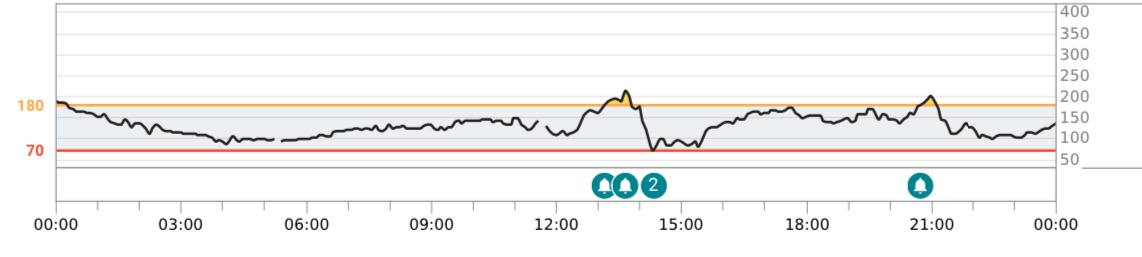
\includegraphics[width=1.0\textwidth]{Images/normal_glucose.jpeg}
    \caption{Normal Glucose Levels}
    \label{fig:normal_glucose}
\end{figure}

\subsection{Example 2: High Glucose Levels}

In the second example, we examine a period where glucose levels were elevated, especially between 03:00 and 06:00. The graph depicts the high glucose peaks.

\begin{figure}[h]
    \centering
    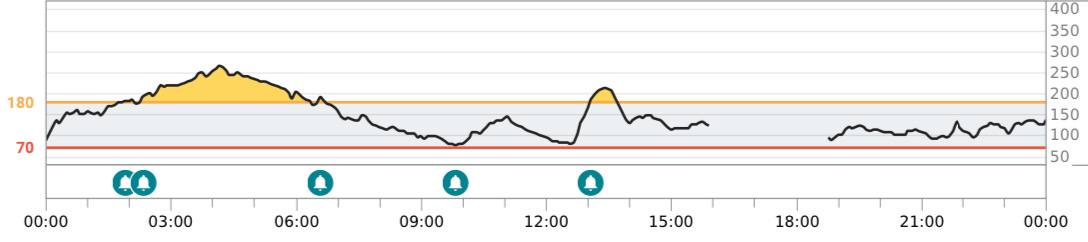
\includegraphics[width=1.0\textwidth]{Images/high_glucose.jpeg}
    \caption{High Glucose Levels}
    \label{fig:high_glucose}
\end{figure}



\subsection{Example 3: Low Glucose Levels}

In the third example, we analyze a period with low glucose levels, mainly occurring during the nighttime hours. The graph highlights fluctuations below the normal threshold.
\pagebreak

\begin{figure}[h]
    \centering
    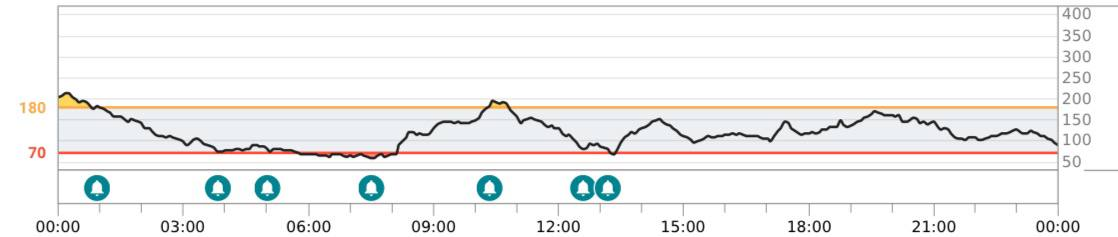
\includegraphics[width=1.0\textwidth]{Images/low_glucose.jpeg}
    \caption{Low Glucose Levels}
    \label{fig:low_glucose}
\end{figure}

These examples demonstrate how analyzing glucose data through our approach can provide significant insights into variations in glucose levels over time, identifying periods of normalcy, high levels, and lows that can be crucial for diabetes management and overall health improvement.


\section{ISEQL}
We have proposed a system based on an extension of relational algebra, ISEQL (Interval-based Surveillance Event Query Language), enriched with powerful temporal operators.
ISEQL significantly enhances the ability to monitor and interpret events in the context of continuous glucose monitoring. For example, it allows:

\begin{itemize}
    \item Rapid identification of prolonged hyperglycemia or hypoglycemia episodes and quantification of their duration and frequency.
    \item Generation of detailed glucose pattern reports to assist doctors in making informed decisions on diabetes management.
\end{itemize}

The integration of ISEQL into our glucose level monitoring system provides a powerful tool for conducting complex temporal analyses more efficiently and robustly, improving the ability to monitor and interpret significant events in glucose data. Through ISEQL, it is also possible to express Allen's interval relations to define high-level models more efficiently.

\subsection{Interval Relations}

We begin by defining an interval relation, which is simply a relation where each tuple is associated with the start and end points of an interval.

\textbf{Definition 4 (Interval Relation).} An interval relation \(R\) is a relation where each tuple \(r = (A, Ts, Te)\) includes attributes \(Ts \in \mathbb{N}\) and \(Te \in \mathbb{N}\), denoting the start and end points of a closed interval. Here, \(A\) is the attribute related to glucose level events in that time interval. We define \(\textit{size}(r) = r.Te - r.Ts\), representing the duration of the event.

The interval denoted by the two points can be written as \([Ts, Te]\) or simply as \(T\). We use a dot (.) to refer to an attribute of a particular tuple: \(r_i.T\) or \(r_i.Ts\). Figure 2 lists the interval relations.

\pagebreak


\begin{figure}[h]
    \centering
    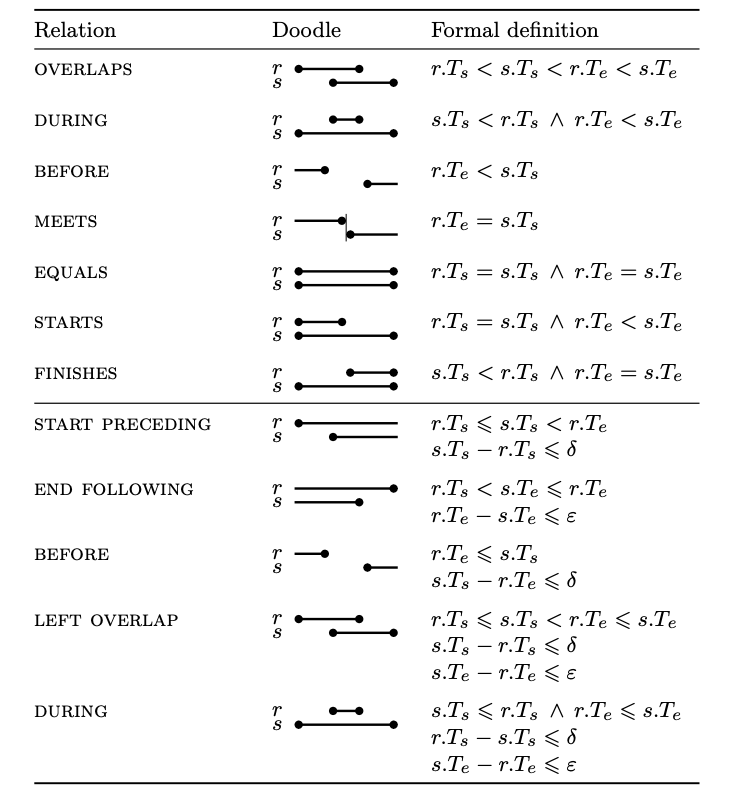
\includegraphics[width=1.0\textwidth]{Images/allen.png}
    \caption{Allen's and ISEQL Interval relations}
    \label{fig:allen}
\end{figure}


\subsection{CARDINALITY CONSTRAINTS}

The \texttt{CARDINALITY CONSTRAINTS} specify the number of occurrences required for a particular interval within the result set of an operation. These constraints are useful for analyzing the frequency of events and filtering results to focus on specific intervals based on their occurrence.

For example, consider two interval relations \(R\) and \(S\), and an interval join operation \(R \omega S\) producing a result set \(\psi\). We can apply cardinality constraints to limit the tuples included in \(\psi\) based on the frequency of intervals from either relation.

\textbf{Definition 5 (Left Cardinality).} Given two interval relations \(R\) and \(S\), tuples \(r_i \in R\) and \(s_j \in S\), an interval join operator \(\omega \in \text{Op}\) with \(\psi = R \omega S\), a standard comparison operator \(\theta'\), and a left cardinality value \(k \in \mathbb{N}\), the constraint is defined as:
\[
R (\theta' k) \omega S = \{\langle r_i, s_j \rangle \in \psi \,|\, r_i \text{ appears in } \psi \text{ the number of times imposed by } \theta' k\}
\]
where \(\theta' \in \{<, \leq, =, \neq, \geq, >\}\).\\



Similarly, the Right Cardinality constraint can be applied to the intervals from the relation \(S\). For example:

\textbf{Definition 6 (Right Cardinality).} Given two interval relations \(R\) and \(S\), tuples \(r_i \in R\) and \(s_j \in S\), an interval join operator \(\omega \in \text{Op}\) with \(\psi = R \omega S\), a standard comparison operator \(\theta'\), and a right cardinality value \(k \in \mathbb{N}\), the constraint is defined as:
\[
R \omega S = \{\langle r_i, s_j \rangle \in \psi \,|\, s_j \text{ appears in } \psi \text{ the number of times imposed by } \theta' k\}
\]
where \(\theta' \in \{<, \leq, =, \neq, \geq, >\}\).\\

By applying both left and right cardinality constraints, the analysis can be further refined, ensuring the inclusion of only the most relevant data points. For instance, if we set \(R (\geq 2) \omega S\), we require that intervals from \(R\) appear at least twice in the result set \(\psi\), highlighting frequent occurrences within the specified analysis parameters.

In the context of glucose monitoring, CARDINALITY CONSTRAINTS can be used to:
\begin{itemize}
    \item Analyze the frequency of specific events, such as anomalies or Time Swings, within a given time frame.
    \item Filter results to focus on intervals that meet or exceed a specified occurrence threshold.
\end{itemize}

\subsection{DURING}

The \texttt{DURING} operator in ISEQL is used to verify if one time interval occurs completely within another. This operator is useful for analyzing the presence and patterns of specific events relative to a broader time interval. In our case we use a varinat of DURING like the DURING JOIN.

The \texttt{DURING JOIN} operator is defined by:
\begin{itemize}
\item $s.T_s \le r.T_s \land r.T_e \le s.T_e$: Interval $r$ starts after or when interval $s$ starts and ends before or when interval $s$ ends.
\item $r.T_s - s.T_s \le \delta$: The difference between the start times of intervals $r$ and $s$ is within a threshold $\delta$.
\item $s.T_e - r.T_e \le \varepsilon$: The difference between the end times of intervals $s$ and $r$ is within a threshold $\varepsilon$.
\end{itemize}

This means that the start time of interval $r$ is greater than or equal to the start time of interval $s$, and the end time of interval $r$ is less than or equal to the end time of interval $s$. Additionally, the difference between the start times of $r$ and $s$ is within a threshold $\delta$, and the difference between the end times of $s$ and $r$ is within a threshold $\varepsilon$.

In the context of High-Level Event Detection, we can use the \texttt{DURING JOIN} operator to:
\begin{itemize}
    \item Identify the occurrence of specific high-level events, such as "Too Frequent Time Swings," within a defined time period (e.g., daily, weekly, monthly, or yearly).
    \item Analyze other high-level events, including significant glucose fluctuations or other patterns, to understand their distribution within specified intervals.
\end{itemize}

The notation for this operator in ISEQL queries is \texttt{DJ}.


\subsection{BEFORE}

The \texttt{BEFORE} operator in ISEQL is used to express a temporal relationship between two intervals, indicating that one interval occurs completely before another interval, without any temporal overlap. This is particularly useful for analyzing the sequence of events in the context of continuous glucose monitoring, allowing the identification of causal or temporal relationships between different glycemic states.

Formally, the \texttt{BEFORE} operator can be defined as:
\begin{itemize}
    \item $r.T_e \le s.T_s$
    \item $s.T_s - r.T_e \le \delta$
\end{itemize}

This means that the end time of interval $r$ is less than or equal to the start time of interval $s$, and the difference between the start time of $s$ and the end time of $r$ is less than or equal to a threshold $\delta$. 

In our context, this allows us to visualize potential Time Swings, such as transitions from hyperglycemia to hypoglycemia and vice versa within a short time frame. The notation for this operator in ISEQL queries is \texttt{Bef}.


\section{Modeling High-Level Events via ISEQL}

The modeling of high-level events in continuous glucose monitoring is crucial for understanding diabetes management and for identifying critical situations that require intervention. ISEQL enables detailed temporal analysis to identify and characterize such events. 

In this context, high-level events can be categorized into two main types: simple events and aggregated events. Simple High-Level Events are characterized by specific temporal attributes and are detected based on straightforward conditions. These events provide fundamental insights into the occurrences and patterns in the glucose data.

Aggregated high-level events, on the other hand, involve the combination of multiple events to analyze broader patterns and trends. By examining the frequency and interactions of events over a specified period, aggregated events offer a more comprehensive view of the data, revealing complex phenomena that may not be apparent from individual events alone.

By leveraging ISEQL's capabilities, both simple and Aggregated High-Level Events can be effectively modeled. This approach allows for a nuanced analysis of glucose data, helping to identify significant changes and trends, thereby supporting better management and intervention strategies in diabetes care.

\subsection{Simple High-Level Events}

Simple High-Level Events are fundamental units of analysis in continuous glucose monitoring. These events are characterized by distinct temporal patterns and are identified through specific conditions applied to the glucose data. By focusing on these basic events, we can gain immediate insights into glucose control and identify critical situations.

To detect these events, we use ISEQL operators such as \texttt{BEFORE}. The \texttt{BEFORE} operator identifies when one event occurs entirely before another event. These tools enhance the analysis and understanding of the temporal relationships between glucose events, allowing for more effective detection of rapid glucose level fluctuations.

\subsubsection{Time Swing}
The concept of \textit{Time Swing} refers to rapid changes in glucose levels that occur over a short period of time. These changes can indicate instability in glucose control and potentially put the patient at risk of complications. Using ISEQL, we can identify these rapid oscillations between hyperglycemic and hypoglycemic intervals.

Detecting \textit{Time Swings} is crucial for monitoring diabetes management. Fast fluctuations in glucose levels may indicate difficulty in maintaining stable control, increasing the risk of complications. The ability to quickly identify \textit{Time Swings} allows for timely intervention and adjustments to the diabetes management plan, preventing episodes of hypoglycemia or hyperglycemia with immediate and serious consequences. Furthermore, accurate monitoring can help identify patterns that require therapeutic adjustments, thereby improving the overall quality of life for the patient.

\pagebreak

\begin{figure}[htb]
    \centering
    \begin{tikzpicture}[relations,xscale=1.4]
        \DrawSpammingTS
    \end{tikzpicture}
    \caption{Time Swing from high to low in one hour}
    \label{fig:Fb}
\end{figure}

We used the \textit{BEFORE} operator to verify that the first interval ends before the second interval begins, thereby identifying a \textit{potential Time Swing}. Specifically, we checked that the hyperglycemic interval ends before the hypoglycemic interval begins (or vice versa), and that the duration between these two intervals is less than the specified time threshold using a \(\delta\) of two hours  to determine if it is indeed a \textit{Time Swing} and not just a \textit{potential Time Swing}. This approach allows us to effectively detect rapid oscillations in glucose levels. In this case we show an example of query to find a Time Swing from high to low or vice versa. 


\begin{align*}
& \pi_{M_1.Patient, M_1.end\_time, M_2.start\_time, M_1.event, M_2.event, (M_2.start\_time - M_1.end\_time) \text{ AS Duration}} \Big( \\
& \quad \sigma_{M_1.Patient = M_2.Patient} \Big( \\
& \quad \quad \Big( \sigma_{M_1.event = \text{"high"}} (M_1) \text{ Bef} (\delta: 2) \sigma_{M_2.event = \text{"low"}} (M_2) \Big) \\
& \quad \quad \text{UNION} \\
& \quad \quad \Big( \sigma_{M_1.event = \text{"low"}} (M_1) \text{ Bef} (\delta: 2) \sigma_{M_2.event = \text{"high"}} (M_2) \Big) \Big) \Big)
\end{align*}


\subsubsection{Too Long Glucose Anomalies}

The \textit{Too Long Glucose Anomalies} events refers to the period during which a patient's glucose level remains outside normal thresholds. Monitoring these events is crucial to understanding how long the patient spends in potentially dangerous conditions.

Measuring the duration of anomalous events is essential for assessing the effectiveness of glycemic control. Too Long periods of hyperglycemia or hypoglycemia may indicate that the current treatment is inadequate and may require therapeutic adjustments.

Prolonged anomalous events are associated with an increased risk of acute and chronic complications. Monitoring their duration allows for timely intervention to reduce the risk of long-term complications.

Using ISEQL, we can determine the duration of each anomalous interval by subtracting the start timestamp (\(tss\)) from the end timestamp (\(tse\)). This data can help identify how long a patient has spent in hyperglycemia or hypoglycemia. A prolonged anomalous event with a duration exceeding the average may indicate an issue in diabetes management that requires attention.

\pagebreak

\begin{figure}[htb]
 \centering
   \begin{tikzpicture}[relations,xscale=1.4]
     \DrawSpammingAD
   \end{tikzpicture}
 \caption{Prolonged glucose anomalies with high glucose for four hours}
 \label{fig:Fb}
\end{figure}

To evaluate these events, we check if the duration exceeds the specific constraint by calculating the difference between the end timestamp and the start timestamp. The constraints used are:

\begin{itemize}
    \item 45 minutes for "extremely high" events,
    \item 1.5 hours for "high" events,
    \item 30 minutes for "low" events,
    \item 10 minutes for "extremely low" events.
\end{itemize}

This approach allows for detailed analysis of prolonged and potentially harmful glucose fluctuations, providing critical insights into patient health.

\begin{align*}
& \pi_{M_1.Patient, M_1.start\_time, M_1.end\_time, M_1.event, (M_1.end\_time - M_1.start\_time) \text{ AS Duration}} \Big( \\
& \quad \sigma_{ \big( \\
& \quad \quad (M_1.event = \text{"extremely high"} \; \text{AND} \; (M_1.end\_time - M_1.start\_time) \geq 45 \text{ minutes}) \; \text{OR} \\
& \quad \quad (M_1.event = \text{"high"} \; \text{AND} \; (M_1.end\_time - M_1.start\_time) \geq 1.5 \text{ hours}) \; \text{OR} \\
& \quad \quad (M_1.event = \text{"low"} \; \text{AND} \; (M_1.end\_time - M_1.start\_time) \geq 30 \text{ minutes}) \; \text{OR} \\
& \quad \quad (M_1.event = \text{"extremely low"} \; \text{AND} \; (M_1.end\_time - M_1.start\_time) \geq 10 \text{ minutes}) \big)} \Big( \\
& \quad \quad \sigma_{M_1.event \in \{\text{"extremely high"}, \text{"high"}, \text{"low"}, \text{"extremely low"}\}} (M_1) \\
& \quad \Big) \Big)
\end{align*}



\subsection{Aggregated High-Level Events}

Aggregated High-Level Events offer a comprehensive view of glucose control by combining multiple high-level events into more complex patterns. These aggregated events are essential for identifying broader trends and making informed decisions about diabetes management.

To analyze these aggregated events, we use ISEQL operators such as \texttt{CARDINALITY CONSTRAINTS}. The \texttt{CARDINALITY CONSTRAINTS} focus on the frequency of events, specifying the minimum number of occurrences needed for an event to be considered significant within a given timeframe. This approach helps in recognizing patterns based on the frequency of certain types of events.

By applying this operator, we can thoroughly analyze the frequency of glucose events, providing a deeper and more actionable understanding of glucose control.

\subsubsection{Too Frequent Glucose Anomalies}

\textit{Too Frequent Glucose Anomalies} refers to the number of times a patient's glucose levels exceed or fall below normal thresholds within a specified period. For our analysis, this period is defined using the Medium-Level event \textit{daily}, which spans from midnight to 23:59. Monitoring these anomalies is crucial for evaluating the stability of glucose control.

Tracking \textit{Too Frequent Glucose Anomalies} helps identify patterns of instability. Frequent hyperglycemic or hypoglycemic events may indicate issues with treatment or other underlying factors. Such anomalies can significantly impact quality of life, potentially increasing the risk of accidents or accelerating diabetic complications.

\begin{figure}[htb]
 \centering
   \begin{tikzpicture}[relations,xscale=1.4]
     \DrawSpammingAF
   \end{tikzpicture}
 \caption{Too Frequent Glucose Anomalies with low glucose for one hour every two hours}
 \label{fig:Fb}
 \end{figure}

In ISEQL, we analyze \textit{Too Frequent Glucose Anomalies} by counting occurrences of hyperglycemic or hypoglycemic intervals within each daily period. The analysis employs:

\begin{itemize}
    \item \textbf{CARDINALITY CONSTRAINTS}: This method ensures that event frequencies meet specified thresholds within daily intervals. Constraints are applied as follows:
    \begin{itemize}
        \item At least 3 occurrences of "high" glucose events,
        \item At least 3 occurrences of "low" glucose events,
        \item At least 2 occurrences of "extremely high" glucose events,
        \item At least 2 occurrences of "extremely low" glucose events.
    \end{itemize}
    
    \item \textbf{DJ (During Join)}: This operator ensures that all counts are correctly aggregated within daily periods.
    
    \item \textbf{DAILY}: This operator determines the daily intervals.
    
    \item \textbf{Union of Results}: This technique combines results from different glucose level checks using a union operation. Each check counts occurrences of a glucose level category within the daily interval, with the \textit{DJ} operator ensuring accurate inclusion of events within each day. The results are then aggregated to provide a comprehensive count of anomalies per day.
\end{itemize}

By employing these methods, we can effectively monitor and analyze \textit{Too Frequent Glucose Anomalies} on a daily basis, thereby enhancing the management of glucose control.

\begin{align*}
& \text{Let } \text{Union\_Results} \text{ be defined as:} \\
& \text{Union} \Bigg( \\
& \quad \pi_{M.event, \text{Count(M.event)} \text{ AS count\_extremely\_high}} \Big( \\
& \quad \quad \sigma_{M.event = \text{"extremely high"}} (M) \;{}^{(\geq 2)} \text{ DJ DAILY} \Big), \\
& \quad \pi_{M.event, \text{Count(M.event)} \text{ AS count\_high}} \Big( \\
& \quad \quad \sigma_{M.event = \text{"high"}} (M) \;{}^{(\geq 3)} \text{ DJ DAILY} \Big), \\
& \quad \pi_{M.event, \text{Count(M.event)} \text{ AS count\_low}} \Big( \\
& \quad \quad \sigma_{M.event = \text{"low"}} (M) \;{}^{(\geq 3)} \text{ DJ DAILY} \Big), \\
& \quad \pi_{M.event, \text{Count(M.event)} \text{ AS count\_extremely\_low}} \Big( \\
& \quad \quad \sigma_{M.event = \text{"extremely low"}} (M) \;{}^{(\geq 2)} \text{ DJ DAILY} \Big) \\
& \quad \Bigg) \\
& \pi_{\text{start\_time\_Time}, \text{end\_time\_Time}, \text{Total\_Count} \text{ AS total\_Count}} \Big( \\
& \quad \text{Count} (\text{Union\_Results}) \Big)
\end{align*}

\subsubsection{Too Frequent Time Swings}

\textit{Too Frequent Time Swings} assesses how often rapid fluctuations in glucose levels, referred to as \textit{Time Swings}, occur within a specified period. A high frequency of these swings may indicate issues with glucose stability, suggesting that the patient’s glucose management might need closer monitoring. Using ISEQL, we can identify and analyze these swings to improve glycemic control and reduce the risk of adverse events.

\pagebreak

\begin{figure}[htb]
    \centering
    \begin{tikzpicture}[relations,xscale=1.4]
        \DrawSpammingTSAF
    \end{tikzpicture}
    \caption{Rapid Time Swings between high and low glucose events within a few hours}  
    \label{fig:Fb}
\end{figure}

To identify \textit{Time Swings}, we use the \textit{BEFORE} operator, which specifies the allowable time gap between successive swings. We then apply \textit{CARDINALITY CONSTRAINTS} to determine how frequently these swings occur. Specifically, the constraint is set to identify instances where at least two Time Swings occur within a specified timeframe.

The analysis focuses on identifying frequent swings from high to low glucose levels or vice versa within the daily interval. The \textit{DAILY} operator defines the daily period for the analysis, while the \textit{DJ (During Join)} operator ensures that swings are accurately aggregated within each day. The \textit{CARDINALITY CONSTRAINTS} are set to require at least two Time Swings within the daily period for swings to be considered frequent.

In summary, the query detects daily Time Swings characterized by rapid glucose changes, using the \textit{BEFORE} with \(\delta\) of tho hours operator to define the time gap and \textit{CARDINALITY CONSTRAINTS} to set the frequency threshold. The results provide insights into the occurrence of these swings and help in evaluating glucose stability and management effectiveness.

\begin{align*}
& \pi_{Patient, \text{Count(*) AS count\_time\_swings}, M_1.event, M_2.event, (M_2.start\_time - M_1.end\_time) \text{ AS Duration}} \Big( \\
& \quad \sigma_{M_1.Patient = M_2.Patient}  \Big( \\
& \quad \quad \big( \sigma_{M_1.event = \text{"high"}} (M_1) \;\text{Bef} (\delta: 2) \; \sigma_{M_2.event = \text{"low"}} (M_2) \\
& \quad \quad \quad \text{UNION} \\
& \quad \quad \big(\sigma_{M_1.event = \text{"low"}} (M_1) \; \text{Bef} (\delta: 2) \; \sigma_{M_2.event = \text{"high"}} (M_2) \big) {}^{(\geq 2)}  \text{DJ DAILY} \Big) 
\end{align*}

\subsubsection{Time Swing With Too Long Glucose Anomalies}

The concept of \textit{Time Swing With Too Long Glucose Anomalies} refers to rapid changes in glucose levels that occur within a short period and overlap with \textit{Too Long Glucose Anomalies} of glycemic events. Using ISEQL, we can identify these rapid oscillations and overlaps between intervals of hyperglycemia and hypoglycemia with abnormal durations.
\pagebreak

\begin{figure}[htb]
    \centering
    \begin{tikzpicture}[relations,xscale=1.4]
        \DrawSpammingTSAD
    \end{tikzpicture}
    \caption{Time Swing from low to high with Too Long Glucose Anomalies on high}
    \label{fig:Fb}
\end{figure}

After identifying the \textit{Time Swings} and \textit{Too Long Glucose Anomalies}, we verify if the patients for these events are the same. Specifically, we check if the patient for the Time Swing events (TS1 and TS2) matches those for the Too Long Glucose Anomalies (TL1 and TL2). We then examine the following two cases:

\begin{itemize}
    \item \textbf{Case 1}: TL1 occurs before TS1. This means that a Too Long Glucose Anomaly (TL1) happens before the Time Swing (TS1).
    \item \textbf{Case 2}: TS2 occurs before TL2. This indicates that a Time Swing (TS2) happens before a Too Long Glucose Anomaly (TL2).
\end{itemize}

By analyzing these cases, we can assess the relationship between rapid glucose changes and prolonged anomalies, providing insights into potential patterns or issues in glucose management.

\begin{align*}
& \pi_{TS.Patient, TS.M2\_event, TS.Duration, AD.Anomalous\_Duration, AD.event} \Big( \\
& \quad \sigma_{TL1.Patient = TS1.Patient \; AND \; TS2.Patient = TL2.Patient} \big( \\
& \quad  \quad TL1 \; \text{Bef}(\delta:0) \; TS1 \; \text{UNION} \; TS2 \; \text{Bef}(\delta:0) \; TL2 \Big) \\
\end{align*}


\section{System Architecture and Diagrams}

The system architecture is designed to be efficient, scalable, and adaptable to changing requirements. It integrates a range of technologies tailored to specific tasks: Laravel for comprehensive web application development, the Flask micro-framework for lightweight web operations, and MySQL for structured and efficient data management. This section provides a detailed overview of the system architecture, emphasizing how these technologies interact and support the overall functionality.

In this section, we will describe three key types of UML diagrams that illustrate different aspects of our system's design:

\begin{itemize}
    \item \textbf{Entity-Relationship (ER) Diagram}: Shows the data structure, including entities, attributes, and relationships. It illustrates how Laravel's ORM and MySQL manage and interact with data.
    \item \textbf{Sequence Diagram}: Depicts the sequence of interactions between various components for different use cases, including how Flask processes requests and how Laravel handles user interactions.
    \item \textbf{Component Diagram:} Highlights the high-level structure of the system, including the main components such as Laravel, Flask, and MySQL, and their interactions within the system.
\end{itemize}

\subsection{Entity-Relationship Diagram}
The ER diagram illustrates the data structure of the system, showing the entities involved and their relationships. MySQL is used to manage the relational database, ensuring data integrity and efficient query processing.



\begin{figure}[h]
\centering
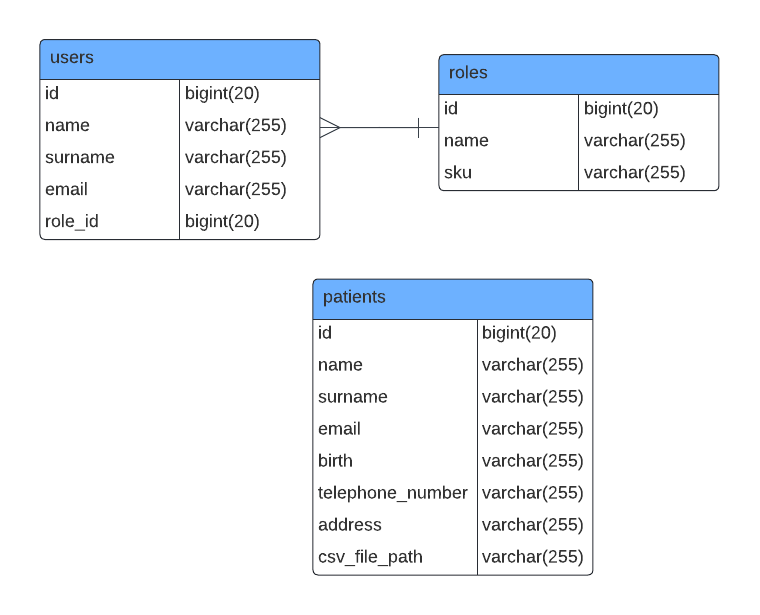
\includegraphics[width=0.8\textwidth]{Images/Diagrams/er.png}
\caption{Entity-Relationship Diagram}
\end{figure}

\subsubsection{Entity Descriptions}
\begin{itemize}
    \item \textbf{Users}: 
    \begin{itemize}
        \item Manages the information of operators/admins.
        \item Stores essential details such as username, password, email, and other personal information.
        \item Each user is associated with a specific role which determines their permissions and access levels within the system.
    \end{itemize}
    
    \item \textbf{Roles}: 
    \begin{itemize}
        \item Defines the different roles available within the system, such as admin, operator, etc.
        \item Each role has specific permissions that dictate what actions a user assigned to that role can perform.
    \end{itemize}
    \item \textbf{Patients}: 
    \begin{itemize}
        \item Contains all the information related to patients.
        \item Includes personal details such as name, date of birth, address, phone number, and the file path of a CSV containing the patient’s glucose level data.
        \item The CSV file is an important component as it provides critical health information for each patient.
    \end{itemize}
\end{itemize}

\subsubsection{Entity-Relationship Description}

There is a one-to-many relationship between \textbf{Roles} and \textbf{Users}. This means that each user is assigned exactly one role, but each role can be assigned to multiple users. This relationship is crucial for managing user permissions and ensuring that each user has the appropriate access level within the system.


\subsection{Sequence Diagrams}
Sequence diagrams describe the flow of operations within the system for various use cases. They provide a detailed view of how components interact over time. Flask handles specific web requests and responses, ensuring seamless communication between the client and the server.

\pagebreak

\begin{figure}[h]
\centering
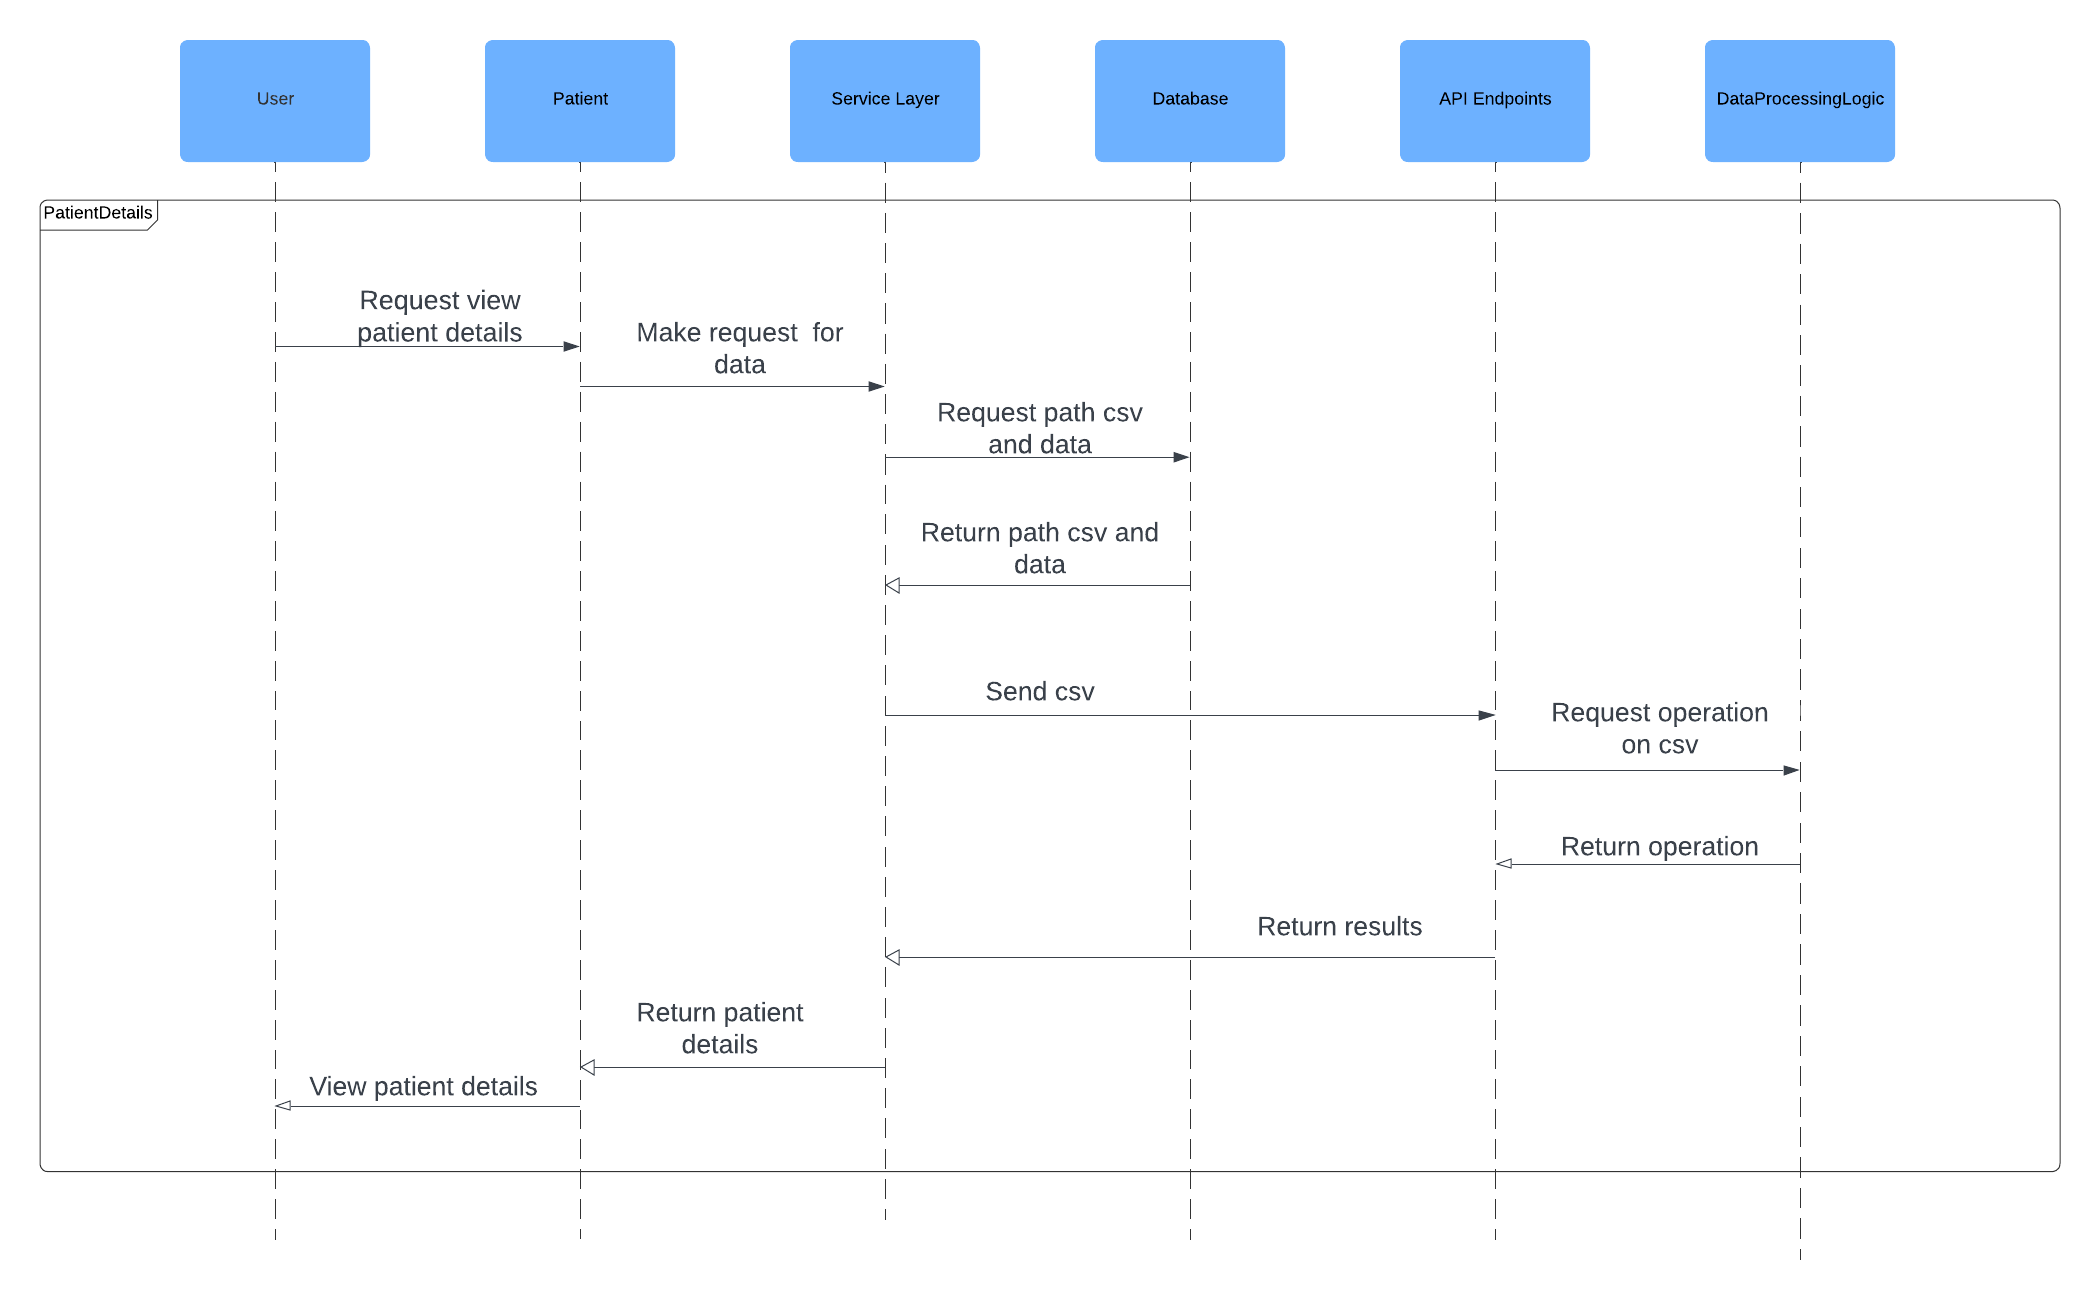
\includegraphics[width=1.0\textwidth]{Images/Diagrams/sequence.png}
\caption{Sequence Diagram for New Patient}
\end{figure}

The user requests to view the details of a patient. This request is forwarded to the service layer, which is responsible for handling the application’s business logic. The service layer requests the patient data and the CSV file path from the database. Upon receiving this information, the service layer uses Flask to send the CSV file to the API Endpoints.

The API Endpoints, in turn, request data processing operations on the CSV file from the Data Processing Logic. Once the processing is complete, the results are sent back to the API Endpoints, which then forward them to the service layer. The service layer compiles all the necessary patient data and forwards it to the patient view, which is displayed to the user.

\subsection{Component Diagram}
The component diagram provides a high-level view of the system's structure, highlighting the various components and their interactions.
\pagebreak
\begin{figure}[h]
\centering
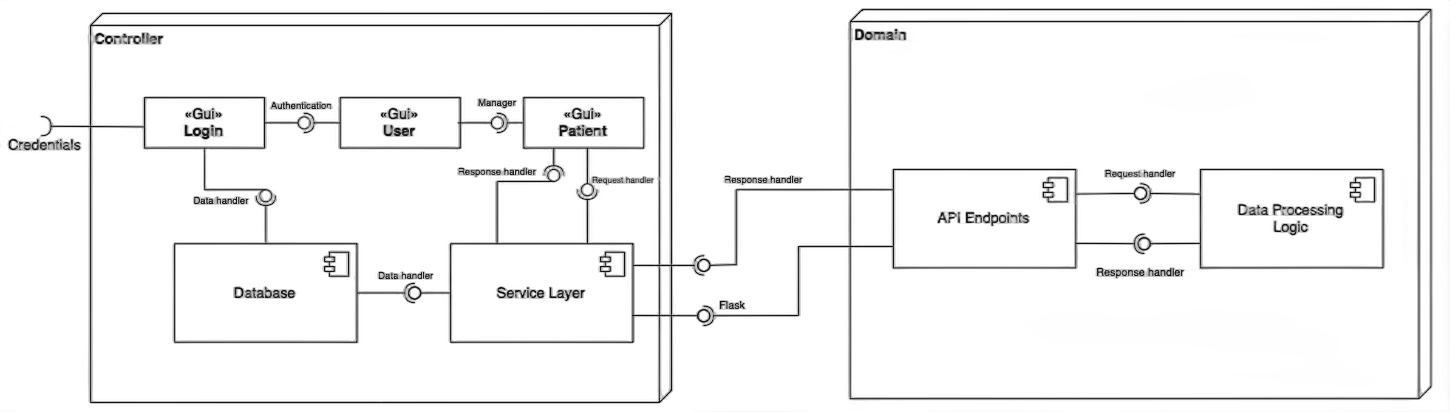
\includegraphics[width=1.0\textwidth,height=0.21\textheight]{Images/Diagrams/component.png}
\caption{System Component Diagram}
\end{figure}


The component diagram highlights the following main areas:

\begin{itemize}
    \item \textbf{Controller Block}:
    \begin{itemize}
        \item \textbf{Login}: Manages user authentication via the \textbf{Database}, verifying credentials and ensuring correct access to the web application.
        \item \textbf{Gui User}: User interface for managing user accounts.
        \item \textbf{Gui Patient}: User interface for viewing and managing patient data. Users request and view patient information through this interface.
        \item \textbf{Service Layer}: Manages business logic and coordinates communications between the \textbf{Database} and the \textbf{API Endpoints}. Interacts with the \textbf{Domain} to request data analysis.
    \end{itemize}
    
    \item \textbf{Domain Block}:
    \begin{itemize}
        \item \textbf{API Endpoints}: Handles data analysis requests received from the \textbf{Service Layer}, forwards them to the \textbf{Data Processing Logic}, and returns the results to the \textbf{Service Layer}.
        \item \textbf{Data Processing Logic}: Performs data analysis operations received from the \textbf{API Endpoints}, using specific classes and methods (e.g., \texttt{IntervalActionDetector}, \texttt{ISEQL}) and returns the results to the \textbf{API Endpoints}.
    \end{itemize}
\end{itemize}

\subsection{Flask Application}

The \textbf{Flask} micro-framework is utilized for handling lightweight web tasks within the system. Flask is chosen for its simplicity and flexibility, allowing quick development and easy integration with other components. It manages specific web requests and responses, particularly for real-time data processing and API endpoints. Flask's minimalistic design makes it ideal for microservices, which handle distinct functionalities such as data extraction, interval action detection, and interaction with the MySQL database. Flask's built-in development server and debugger also facilitate a smooth development process.

\subsection{Laravel Framework}

The \textbf{Laravel} framework is used as the primary technology for building and maintaining the web application. Laravel offers a comprehensive suite of tools and libraries that streamline development, including an expressive ORM (Eloquent), powerful templating engine (Blade), and robust routing capabilities. Laravel's modular packaging system and extensive ecosystem allow easy integration of additional functionalities. It also provides built-in features for authentication, authorization, and session management, ensuring a secure and maintainable codebase. The framework's emphasis on elegant syntax and developer productivity makes it an excellent choice for large-scale web applications.

\subsection{Database Management}

The website's data is managed using \textbf{MySQL}, a robust relational database management system. We utilize \textbf{PhpMyAdmin}, a web-based interface for MySQL, to administer the database. PhpMyAdmin simplifies tasks such as creating databases, managing tables, and executing SQL queries directly through a user-friendly interface.

The database stores various types of information critical to the website's functionality, including user credentials, patient data, and system configurations. Laravel's ORM (Object-Relational Mapping) capabilities streamline database interactions, allowing developers to define database schema and perform database operations using PHP syntax.

PhpMyAdmin also facilitates database backups, ensuring data integrity and disaster recovery readiness. This comprehensive database management setup ensures reliable storage and efficient retrieval of glucose data for analysis and visualization within the website.


\section{Implementation}

In this section, we explore the implementation of glucose data analysis using \textbf{Python} and the pandas library. \textbf{Pandas} is a powerful library for data manipulation and analysis, offering high-level data structures and a wide range of tools for dataset management. We use a CSV file containing glucose data from the past 90 days, specifically from February 13, 2024, to May 12, 2024. including essential time-related information for monitoring and analyzing blood glucose level variations.

\subsection{Project Structure}

The project is organized into several files, each with a specific role in the glucose data analysis pipeline:
\pagebreak
\begin{itemize}
    \item \textbf{interval\_action\_detector.py}:
    \begin{itemize}
        \item Contains the \texttt{IntervalActionDetector} class, responsible for analyzing glucose data. This class includes the method \texttt{offline\_interval
        \_action\_detection}, which categorizes glucose levels and identifies intervals based on predefined thresholds.
    \end{itemize}
    
    \item \textbf{interval.py}:
    \begin{itemize}
        \item Defines the \texttt{Interval} class. This class represents a time interval with a start and end time, along with associated glucose level events and their duration.
    \end{itemize}
    
    \item \textbf{iseql.py}:
    \begin{itemize}
        \item Contains the \texttt{ISEQL} class. This class is used for further analysis of the intervals, such as detecting Too Long Glucose Anomalies and Too Frequency, finding Time Swings, and other advanced analyses.
    \end{itemize}
    
    \item \textbf{data\_processing\_logic.py}:
    \begin{itemize}
        \item Implements a Flask web application to provide an API endpoint for processing glucose data. This file facilitates the interaction with the analysis logic and can be integrated with Laravel or any other front-end framework to create a comprehensive web application.
    \end{itemize}
    
    \item \textbf{analysis.py}:
    \begin{itemize}
        \item This file contains code for evaluating the performance and scalability of the glucose data analysis pipeline. It includes tools to test the efficiency of various operations, measure execution times, and assess how the system handles increasingly larger datasets.
    \end{itemize}
\end{itemize}

\subsection{Data Extraction}

To analyze glucose data, we extract relevant information from daily logs. Using pandas, we load data from a CSV file that includes significant columns such as event type, subtype, date, time of each measurement, and glucose value in mg/dL. This allows us to focus on pertinent columns for analysis.

\subsection{IntervalActionDetector Class}

In our glucose data analysis, we have implemented the class IntervalActionDetector with a function called \texttt{offline\_interval\_action\_detection} to create time intervals associated with different glucose levels in the dataset. This function is designed to automatically identify and label intervals based on detected glucose levels.

The function takes input from a DataFrame \texttt{glucose\_data} containing glucose level data, along with various predefined thresholds to categorize glucose levels as high, low, or extremely low. By iterating through the first 10,000 records of the DataFrame, the function analyzes each glucose measurement and determines its glucose level category.

Key threshold parameters include:
\begin{itemize}
    \item \texttt{extreme\_high\_threshold}: Threshold for extremely high glucose level.
    \item \texttt{high\_threshold}: Threshold for high glucose level.
    \item \texttt{low\_threshold}: Threshold for low glucose level.
    \item \texttt{extreme\_low\_threshold}: Threshold for extremely low glucose level.
\end{itemize}

During iteration, the function evaluates each glucose measurement against the defined thresholds and assigns a corresponding event label such as 'extremely high', 'high', 'extremely low', 'low', or 'normal'. Time intervals are then created based on significant changes in detected events.

This methodology segments and clearly visualizes periods of high, low, or extremely low glucose levels over time, enabling in-depth analysis of glucose level variations and related intervention actions.

\subsection{Interval Class}
The \texttt{Interval} class represents a time interval associated with a specific glucose event. Each instance of \texttt{Interval} includes the following properties:
\begin{itemize}
    \item \texttt{symbol}: Identifying symbol for the event.
    \item \texttt{start\_time} and \texttt{end\_time}: start\_time and end time of the interval.
    \item \texttt{event}: Type of glucose event ('extremely\_high', 'high', 'normal', 'low', 'extremely\_low').
    \item \texttt{duration}: Interval duration, automatically calculated if not specified.
\end{itemize}

\subsection{ISEQL Class}
The \texttt{ISEQL} class manages a collection of time intervals (\texttt{intervals}). It provides useful methods to add, retrieve, and filter intervals, manage ISEQL relations, and find all high-level events.

Primary methods for interval management include:
\begin{itemize}
    \item \texttt{add\_interval(interval)}: Adds an interval to the collection.
    \item \texttt{get\_intervals()}: Retrieves all intervals.
    \item \texttt{find\_event\_interval(event\_name)}: Finds a specific interval based on the event type.
    \item \texttt{check\_anomalies\_event(interval)}: Checks if the interval is anomalous.
    \item \texttt{create\_daily\_intervals()}: Creates and returns a dictionary of daily intervals.
\end{itemize}

Subsequently, methods were implemented for ISEQL relations:
\begin{itemize}

    \item \texttt{DURING(interval1, interval2)}: Checks if the first interval occurs completely during the second interval.
    \item \texttt{BEFORE(interval1, interval2, delta)}: Checks if the first interval ends before the start of the second interval, considering a time delta margin.
    \item \texttt{CARDINALITY\_CONSTRAINTS(intervals, event, min\_count)}: Checks if the number of intervals with a specific level within a given time frame meets the minimum count.
\end{itemize}

Finally, the following methods were implemented to find and manage high-level events:
\begin{itemize}
     \item \texttt{find\_time\_swing(time\_threshold=timedelta(hours=2))}: Detects Time Swing, which are significant changes in glucose levels occurring within a defined time interval.
    \item \texttt{find\_too\_frequent\_glucose\_anomalies(min\_high=3, min\_low=3, min\_extremely\_high=2, min\_extremely\_low=2)}: Identifies days with significant anomalies in the frequency of glucose level events.
    \item \texttt{find\_too\_frequent\_time\_swings(time\_swing\_threshold=timedelta(hours=2), min\_ts=2)}: Finds significant glucose level changes that occur too frequently within a specified time period.
    \item \texttt{find\_too\_long\_glucose\_anomalies()}: Identifies time intervals where glucose levels show significant duration anomalies.
    \item \texttt{find\_time\_swing\_with\_too\_long\_glucose\_anomalies()}: Finds Time Swings that are associated with Too Long Glucose Anomalies intervals.
\end{itemize}

\subsection{Data Processing Logic}

The data processing logic is implemented in the file \texttt{data\_processing\_logic.py}, which configures a Flask application to handle incoming CSV files and analyze glucose data. The main functionality is encapsulated in the \texttt{/process-csv} endpoint. Below is an overview of its operations:

\begin{itemize}
    \item \textbf{File Handling}:
    \begin{itemize}
        \item The endpoint receives a CSV file from the client. The file is saved in a predefined directory and a pandas DataFrame is created by reading this file.
        \item If an error occurs during file handling or reading, an appropriate error message is returned to the client.
    \end{itemize}
    
    \item \textbf{Data Preprocessing}:
    \begin{itemize}
        \item Relevant columns are selected from the DataFrame and initial rows are skipped to clean the data. This preprocessing ensures that only the necessary data is retained for analysis.
    \end{itemize}
    
    \item \textbf{Interval Detection}:
    \begin{itemize}
        \item An instance of the \texttt{IntervalActionDetector} class is created to process the cleaned glucose data.
        \item The \texttt{offline\_interval\_action\_detection} method is used to categorize glucose levels and identify periods of interest.
    \end{itemize}
    
    \item \textbf{Interval Management}:
    \begin{itemize}
        \item The detected intervals are stored in instances of the \texttt{Interval} class, which are then added to an instance of \texttt{ISEQL}.
        \item The \texttt{ISEQL} class is used to manage these intervals and perform various analyses, including searching for anomalies and glucose fluctuations.
    \end{itemize}
    
    \item \textbf{Results Analysis and Formatting}:
    \begin{itemize}
        \item Several analysis methods from the \texttt{ISEQL} class are called to detect anomalies and significant patterns in the glucose data.
        \item The results are formatted into a structured JSON response, including details on anomalous frequencies, durations, glucose fluctuations, and more.
        \item Utility functions such as \texttt{format\_duration}, \texttt{format\_datetime}, and \texttt{format\_day} are used to ensure that the output is user-readable.
    \end{itemize}
    
    \item \textbf{Additional Analysis}:
    \begin{itemize}
        \item The \texttt{analyze\_glucose\_data} function from the \texttt{analysis} module is called to perform additional analysis on the intervals. The results from this function are included in the final JSON response.
    \end{itemize}
    
    \item \textbf{Endpoint Execution}:
    \begin{itemize}
        \item The Flask application is run with debugging enabled, allowing real-time feedback and easier troubleshooting.
    \end{itemize}
\end{itemize}

This setup ensures that glucose data is processed efficiently and effectively, providing meaningful insights into glucose levels and trends. The Flask application acts as a bridge between raw data and analytical insights, facilitating the integration of data processing into larger systems or applications.

For a detailed explanation of the results and the analyses performed, please refer to Section \ref{sec:result_analysis}.


\subsection{Website Development}

In the implementation phase, the website integrates \textbf{Laravel} and \textbf{Flask} to provide a comprehensive solution for web application development and data processing. 

Laravel handles the core functionalities of the web application, including user authentication, data management, and interaction with the MySQL database. It utilizes its ORM (Eloquent) to manage database operations and streamline development.

For specialized data processing tasks, such as analyzing glucose data, we employ a Flask application. Defined in the file \textbf{data\_processing\_login.py}, Flask provides API endpoints for processing data, managing HTTP requests, and returning results in JSON format. Flask receives data from Laravel, performs the necessary computations, and returns the processed results.

This integration of Laravel and Flask ensures effective data handling and processing, while PhpMyAdmin is used for managing backups and ensuring data integrity.


\subsubsection{Login}
The login functionality is a crucial part of the website's user management system. It ensures that only authorized users can access the system and its functionalities. The login page will use Laravel's built-in authentication mechanisms to handle user sign-in.

Users will be prompted to enter their credentials (username and password) on the login page. Upon successful authentication, they will be redirected to the dashboard.

The login page will include "Forgot Password" to enhance user security.

\begin{figure}[h!]
    \centering
    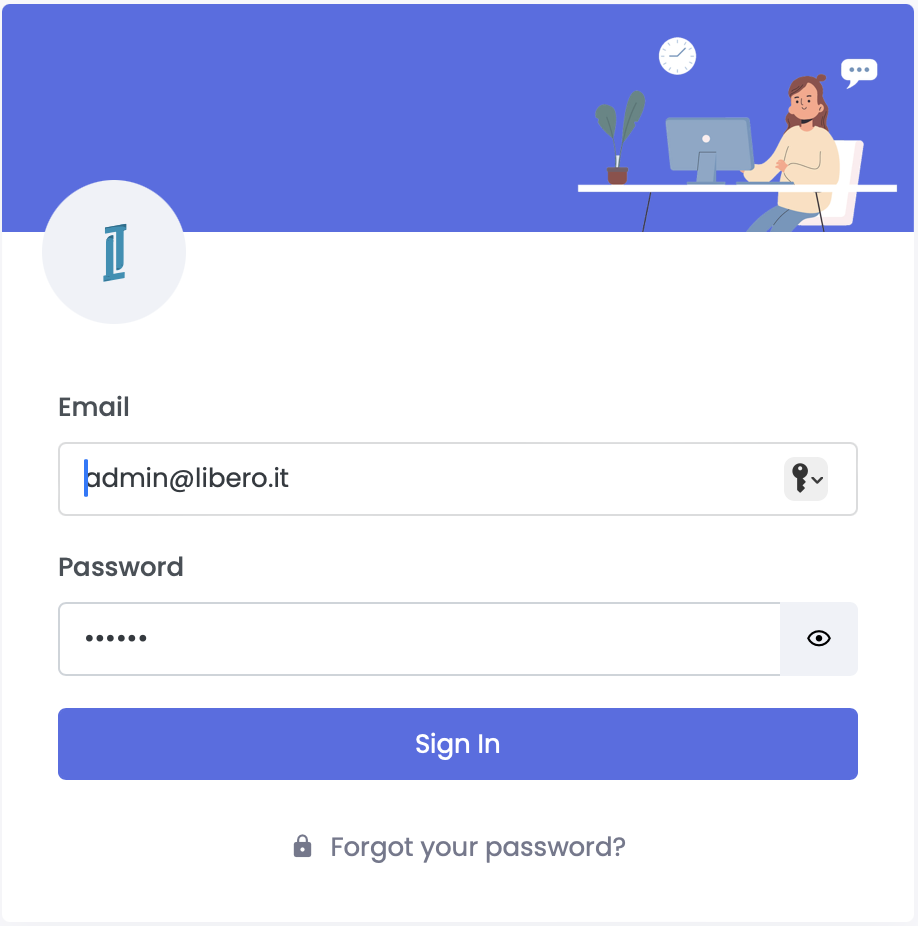
\includegraphics[width=0.5\textwidth]{Images/Web/login.png}
    \caption{Login}
    \label{fig:login_screen}
\end{figure}

\pagebreak

\subsubsection{User Management}
The website will feature user authentication and authorization functionalities using Laravel's built-in authentication system. Users will be categorized into two main roles:

\begin{itemize}
    \item \textbf{Admin}: Admin users have full access to all functionalities of the website. They can manage operators (create, edit, delete), view patient data, and perform administrative tasks. By default, there is a principal admin who has the authority to modify and delete other admins and change their roles (Admin or Operator).
    \item \textbf{Operator}: Operators have restricted access compared to admins. They can view patient data and perform data analysis tasks but cannot manage other users.
\end{itemize}



\subsubsection{Dashboard}
The dashboard serves as the main interface upon logging into the website. It provides an overview of key metrics such as statistics on the number of operators, patients, and CSV files uploaded, as well as the latest operators added. The dashboard is customizable based on user preferences and provides interactive visualizations for deeper insights into patient data.

\begin{figure}[h!]
    \centering
    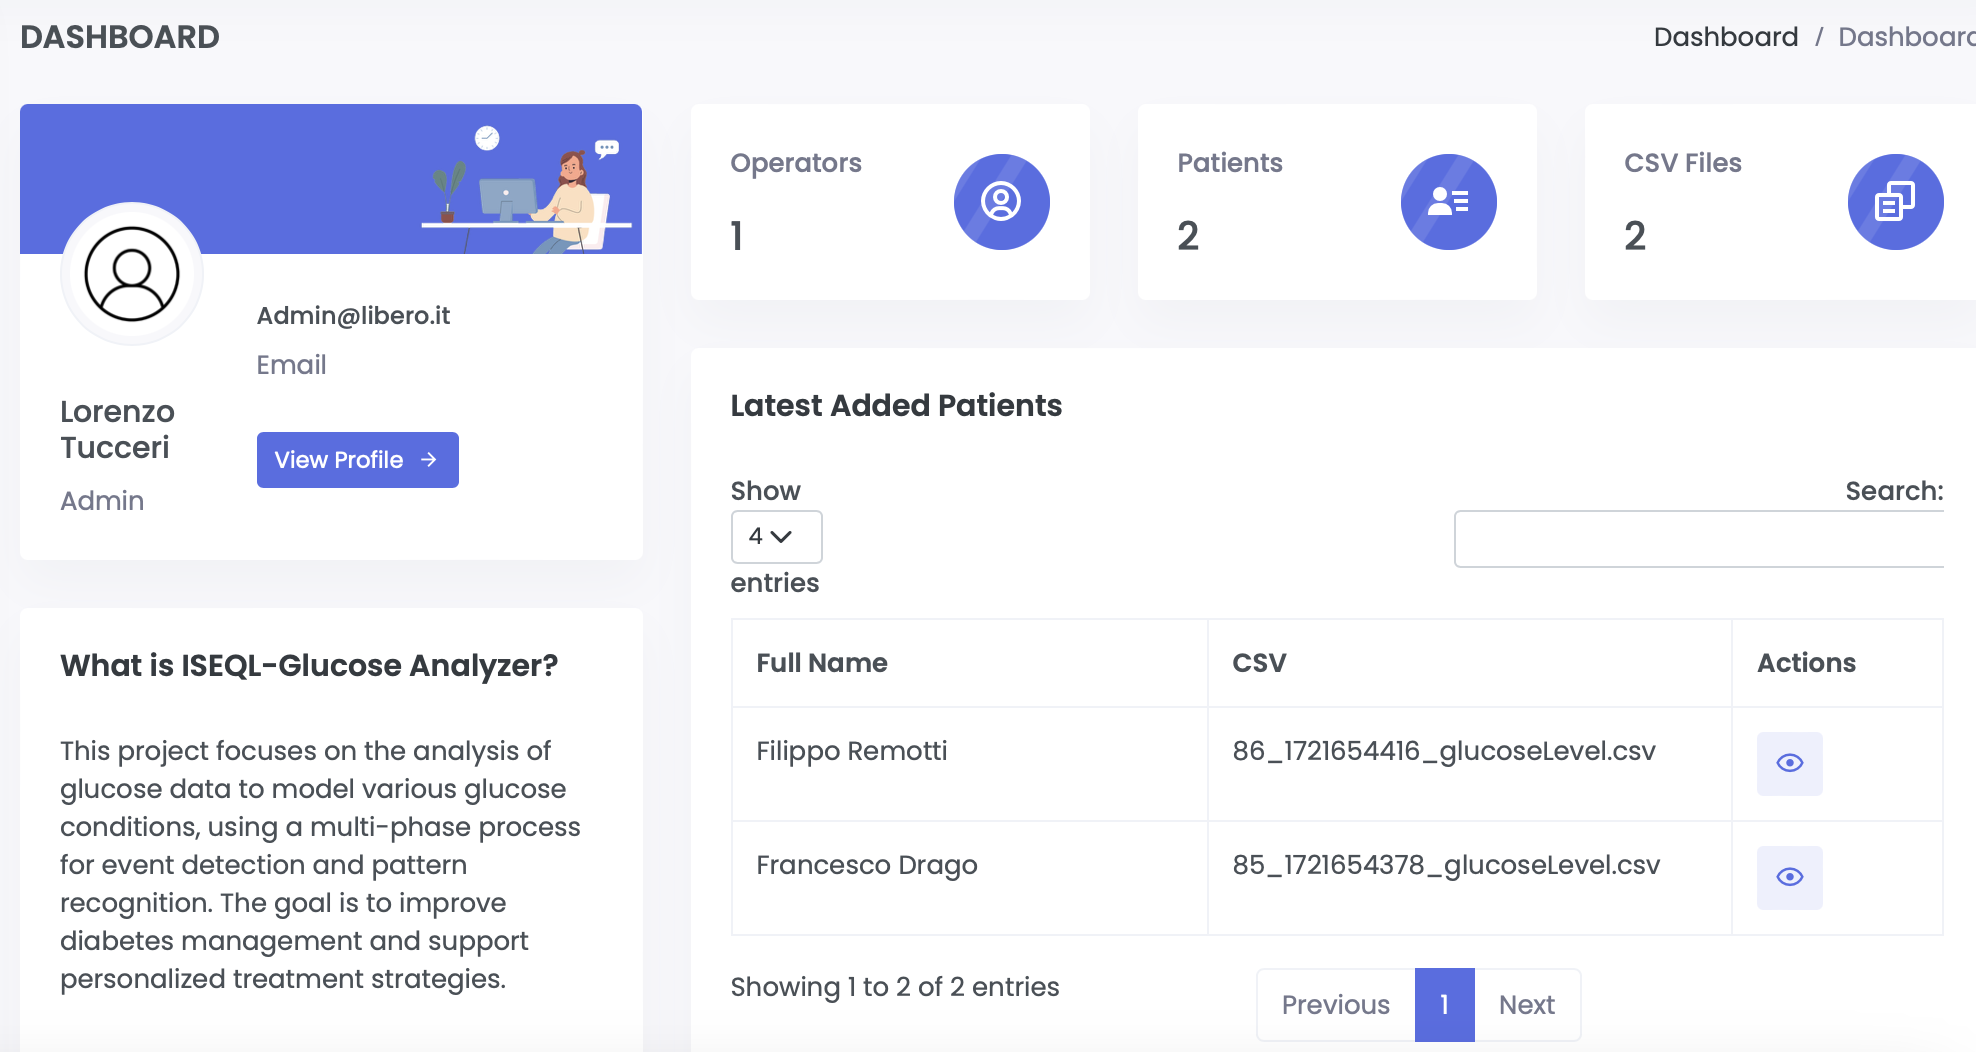
\includegraphics[width=0.8\textwidth]{Images/Web/dashboard.png}
    \caption{Dashboard}
    \label{fig:Dashboard}
\end{figure}

\pagebreak
\subsubsection{Profile and Operator Management}
Users, both admins and operators, can manage their profiles through dedicated settings. They can update personal information, change passwords, and adjust notification preferences. Admin users also have access to a separate section for managing operators, where they can add new operators, modify existing profiles, and delete accounts if necessary.


\begin{figure}[h!]
    \centering
    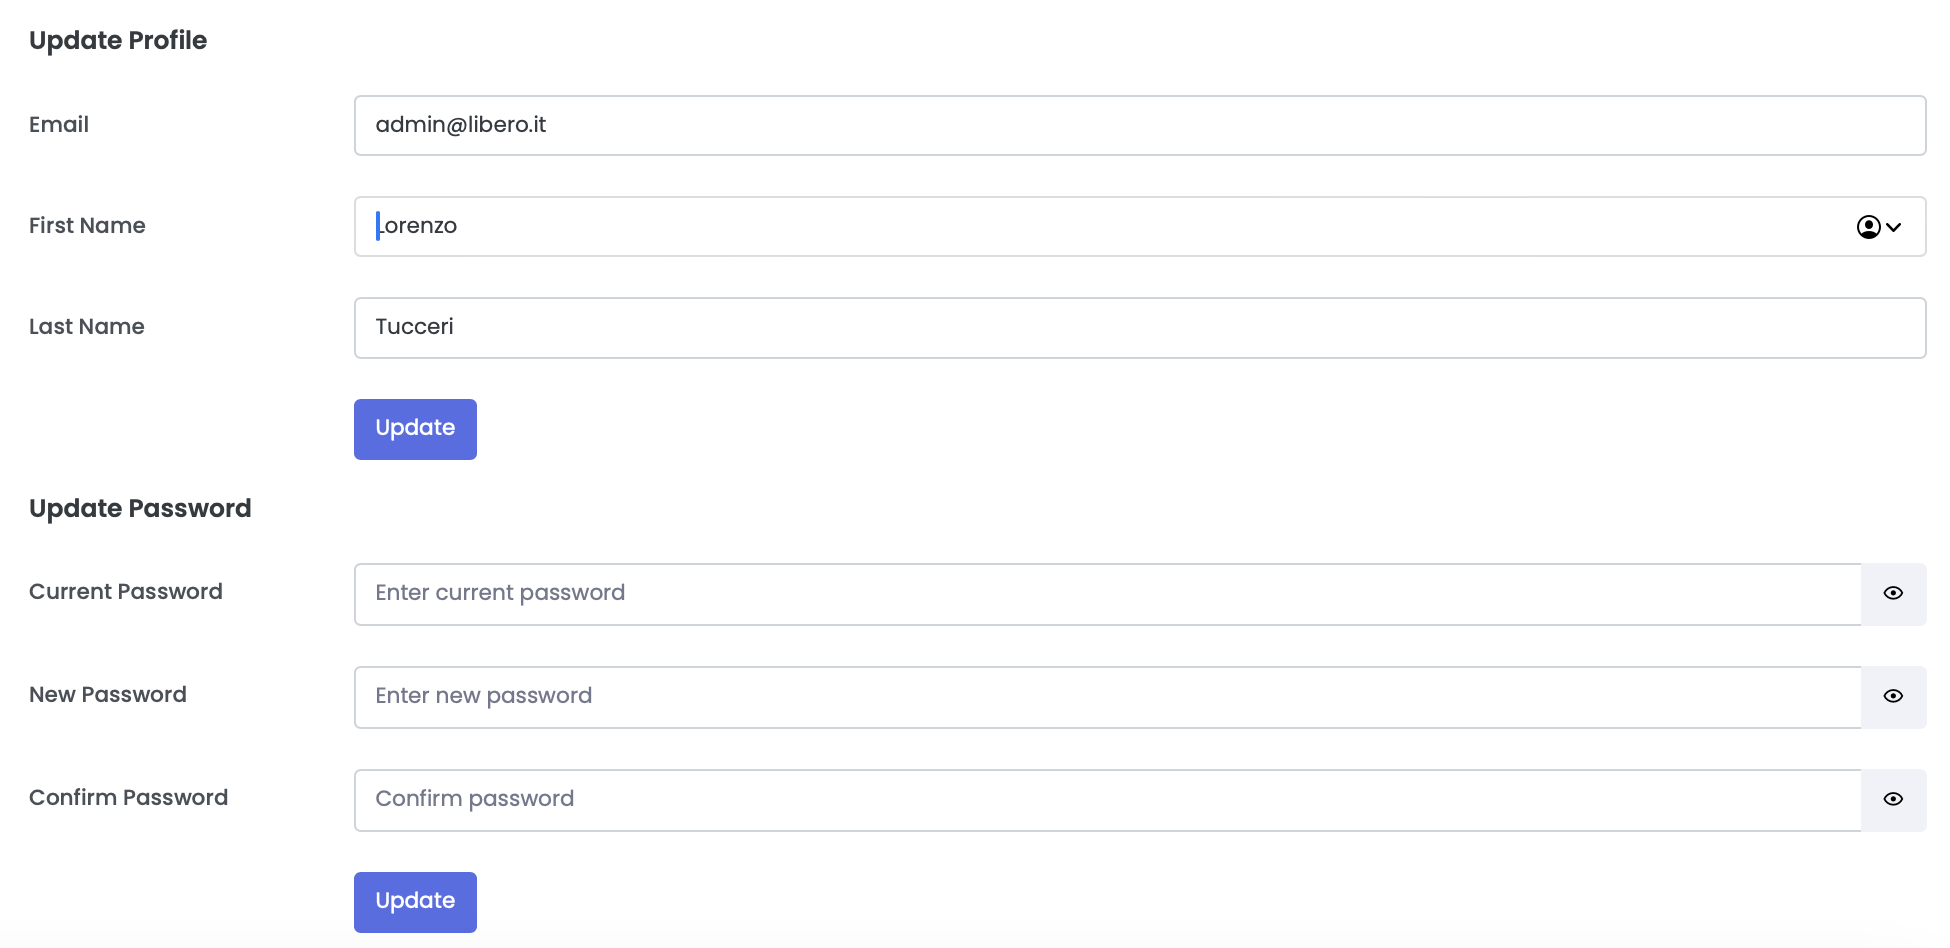
\includegraphics[width=0.8\textwidth]{Images/Web/personal_profile.png}
    \caption{Personal profile}
    \label{fig:Personal profile}
\end{figure}


\subsubsection{Patient Management}
The website includes functionalities for managing patient records and data. Admins and operators can add new patients to the system, update patient information, and view detailed glucose data for each patient. Additionally, for each patient, CSV files containing their glucose data can be uploaded for studies and analysis.

\begin{figure}[h!]
    \centering
    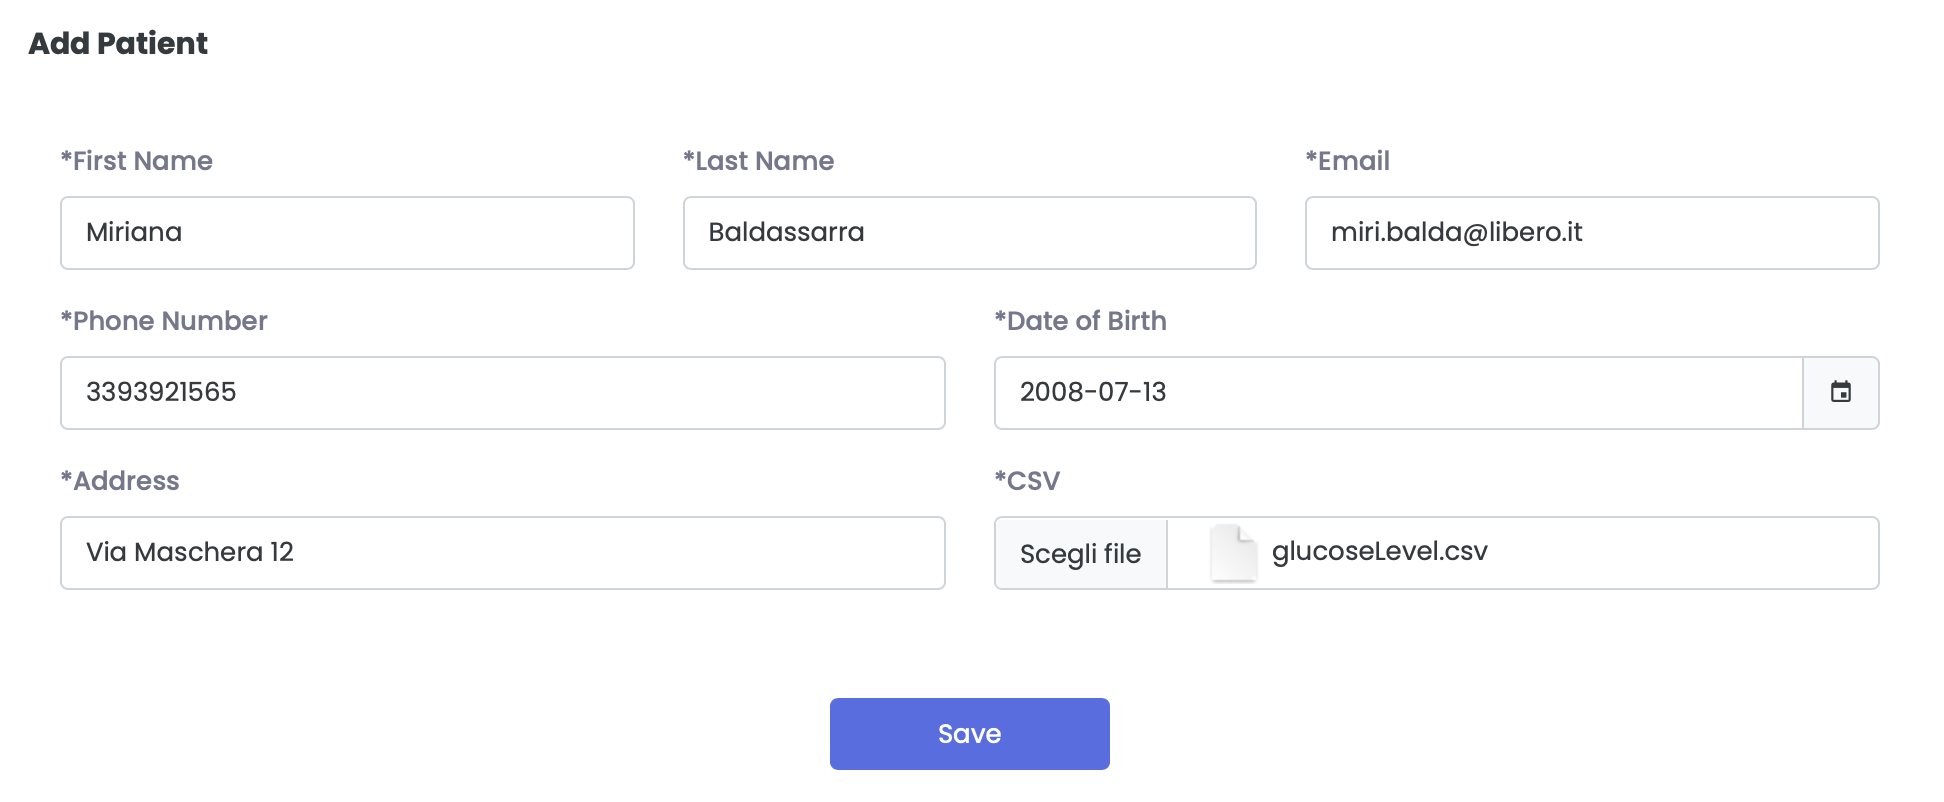
\includegraphics[width=0.8\textwidth]{Images/Web/new_patient.png}
    \caption{New patient}
    \label{fig:New Patient}
\end{figure}

In this subsection, we have detailed patient information; all statistics and results from the uploaded CSV file are displayed. This includes metrics such as Time Swing, high glucose levels, low glucose levels, and other relevant data points derived from the glucose records. Additionally, it will be possible to download a PDF containing all the data related to the patient.

\begin{figure}[h!]
    \centering
    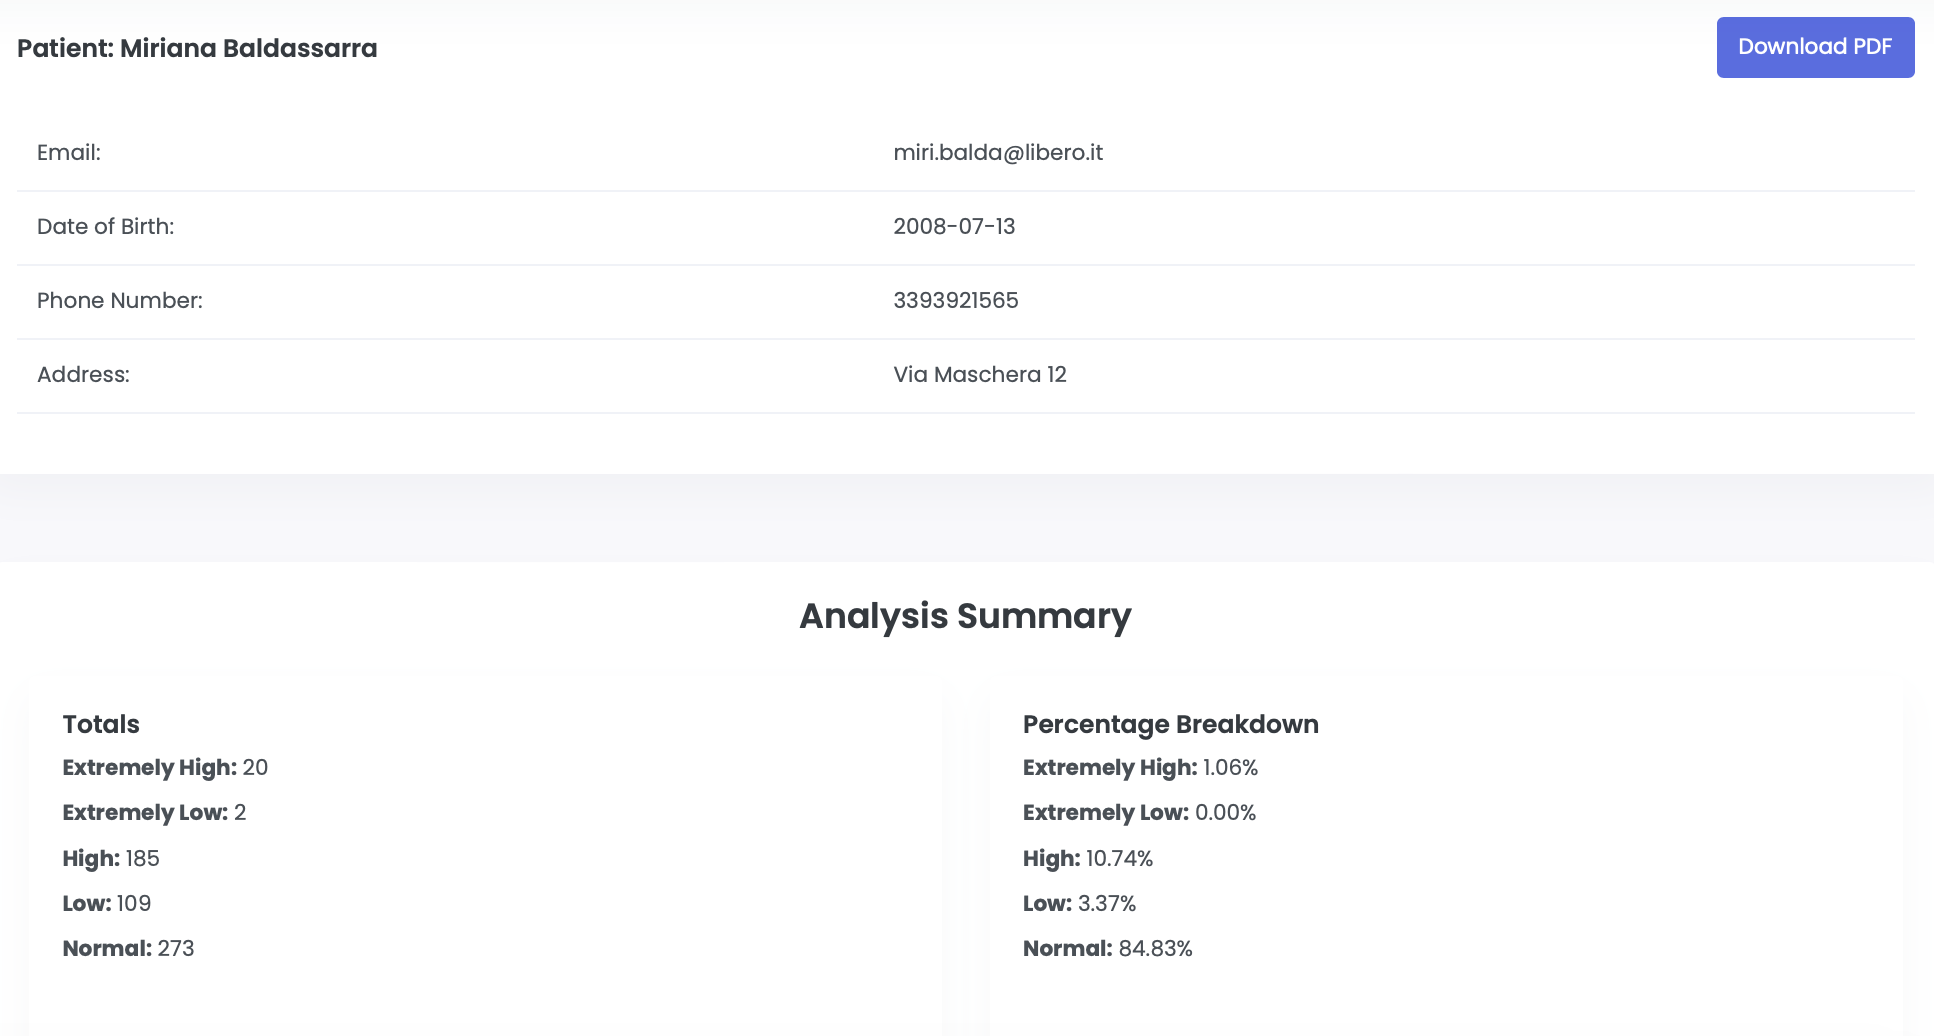
\includegraphics[width=0.8\textwidth]{Images/Web/detail_patient.png}
    \caption{Patient Details}
    \label{fig:Patient Details}
\end{figure}

\subsubsection{Website Limitations}

In this version, the website enforces a restriction of one CSV file per patient, simplifying data management but potentially limiting in-depth analysis. Currently, the platform lacks graphical representations to visualize data trends and events. While detailed information is available in the patient detail section, the absence of charts may hinder the clarity and interpretability of glucose data and associated metrics. Additionally, the application only accepts CSV files exported from Dexcom.

\section{Result and Analysis}
\label{sec:result_analysis}
In this section, we present the results obtained from analyzing glucose data using the functions and classes implemented in the file \texttt{analysis.py}. We evaluated the glycemic data by identifying extremely high, high, low, and extremely low glucose levels based on predefined thresholds and segmented these data into time intervals for detailed analysis.


\subsection{General Statistics}

The general statistics of the analyzed glucose data are as follows:

\begin{itemize}
    \item \textbf{Total Counts:}
    \begin{itemize}
        \item Extremely High: 20
        \item High: 185
        \item Low: 109
        \item Extremely Low: 2
        \item Normal: 273
    \end{itemize}
    
    \item \textbf{Total Durations:}
    \begin{itemize}
        \item Extremely High: 08:20
        \item High: 84:30
        \item Low: 26:33
        \item Extremely Low: 00:00
        \item Normal: 667:44, representing 84.83\% of the total time.

    \end{itemize}

\end{itemize}

These statistics provide an overview of the distribution and duration of different glucose level events within the dataset.


\subsection{Simple High-Level Event}

The \texttt{find\_time\_swing} function identified significant changes in glucose levels, characterized by rapid fluctuations between high and low glucose levels. The results are as follows:

\begin{itemize}
    \item A total of 39 significant Time Swings were detected.
\end{itemize}

This indicates that significant Time Swings are frequent and often lead to periods of prolonged instability.

\subsection{Aggregated High-Level Event}

In this subsection, we analyze various aspects related to aggregation high-level anomalous events, with a focus on Too Frequent Glucose Anomalies, Too Frequent Time Swings, Too Long Glucose Anomalies, and Time Swings With Too Long Glucose Anomalies.

\subsubsection{Too Frequent Glucose Anomalies}

The \texttt{find\_too\_frequent\_glucose\_anomalies } function revealed the day with the highest number of anomalies:

\begin{itemize}
    \item On February 23, 2024, 3 high glucose events, 13 low glucose events, 0 extremely high glucose events, and 1 extremely low glucose event were recorded, totaling 17 anomalous events.
\end{itemize}

This highlights specific days when glucose levels were particularly unstable.

\subsubsection{Too Frequent Time Swings}

The analysis of Time Swings revealed:

\begin{itemize}
    \item There are 7 days with too frequent time swings, amounting to 19 time swings.
    \item These account for 17.95\% of the total Time Swings detected.
\end{itemize}

This indicates that some Time Swings occur with such frequency that they may warrant closer monitoring.

\subsubsection{Too Long Glucose Anomalies}

The \texttt{find\_too\_long\_glucose\_anomalies} function showed:

\begin{itemize}
    \item For extremely high glucose intervals, 1.06\% exhibited Too Long Glucose Anomalies.
    \item For high glucose intervals, 10.74\% exhibited Too Long Glucose Anomalies.
    \item For low glucose intervals, 3.37\% exhibited Too Long Glucose Anomalies.
    \item Extremely low glucose intervals showed 0.00\% Too Long Glucose Anomalies.

\end{itemize}

The duration data highlights which glucose levels are more prone to anomalies and requires specific attention.

\subsubsection{Time Swings With Too Long Glucose Anomalies}

The analysis of Time Swings and their duration yielded:

\begin{itemize}
    \item A total of 11 Time Swings were found to have Too Long Glucose Anomalies.
    \item This represents 28.21\% of all Time Swings detected.
\end{itemize}

This suggests that a significant portion of Time Swings is associated with periods of Too Long Glucose Anomalies, emphasizing the need to address prolonged instability in glucose levels.

These observations collectively offer insights into the patterns and anomalies in glucose levels, enabling targeted interventions to manage and mitigate fluctuations effectively.

\subsection{Evaluation Metrics}

In this subsection, evaluation metrics such as efficiency, precision, recall, etc., will be added.

Here's the updated section with the provided data:

\subsection{Scalability and Efficiency}

The analysis of scalability and efficiency was conducted using datasets of varying sizes: 25\%, 50\%, 75\%, and 100\% of the total dataset. The following results summarize execution times and growth rates for different methods:

\subsubsection{Execution Times}

Table \ref{tab:execution_times} presents the execution times for each method at different dataset sizes.


\begin{table}[h!]
\centering
\begin{tabular}{|l|r|r|r|r|}
\hline
\textbf{Method} & \textbf{25\%} & \textbf{50\%} & \textbf{75\%} & \textbf{100\%} \\
\hline
\texttt{offline\_interval\_action\_detection} & 0.1405 & 0.1936 & 0.1950 & 0.1940 \\
\texttt{find\_time\_swings} & 0.00007 & 0.00012 & 0.00012 & 0.00012 \\
\texttt{find\_too\_frequent\_glucose\_anomalies} & 0.00014 & 0.00022 & 0.00021 & 0.00022 \\
\texttt{find\_too\_frequent\_time\_swings} & 0.00117 & 0.00282 & 0.00281 & 0.00281 \\
\texttt{find\_too\_long\_glucose\_anomalies} & 0.00002 & 0.00003 & 0.00003 & 0.00003 \\
\texttt{find\_time\_swing\_with\_too\_long\_glucose\_anomalies} & 0.00012 & 0.00022 & 0.00022 & 0.00022 \\
\hline
\end{tabular}
\caption{Execution Times for Different Methods}
\label{tab:execution_times}
\end{table}


\subsubsection{Average Execution Times}

Table \ref{tab:avg_execution_times} shows the average execution times for each method across all dataset sizes.

\begin{table}[h!]
\centering
\begin{tabular}{|l|r|}
\hline
\textbf{Method} & \textbf{Average Time (seconds)} \\
\hline
\texttt{offline\_interval\_action\_detection} & 0.18076124 \\
\texttt{find\_time\_swings} & 0.00011016 \\
\texttt{find\_too\_frequent\_glucose\_anomalies} & 0.00019583 \\
\texttt{find\_too\_frequent\_time\_swings} & 0.00240318 \\
\texttt{find\_too\_long\_glucose\_anomalies} & 0.00002658 \\
\texttt{find\_time\_swing\_with\_too\_long\_glucose\_anomalies} & 0.00019381 \\
\hline
\end{tabular}
\caption{Average Execution Times}
\label{tab:avg_execution_times}
\end{table}
\pagebreak
\subsubsection{Average Growth Rates}

Table \ref{tab:avg_growth_rates} provides the average growth rates of execution times as the dataset size increases.

\begin{table}[h!]
\centering
\begin{tabular}{|l|r|}
\hline
\textbf{Method} & \textbf{Average Growth Rate} \\
\hline
\texttt{offline\_interval\_action\_detection} & 0.1267 \\
\texttt{find\_time\_swings} & 0.2431 \\
\texttt{find\_too\_frequent\_glucose\_anomalies} & 0.1968 \\
\texttt{find\_too\_frequent\_time\_swings} & 0.4690 \\
\texttt{find\_too\_long\_glucose\_anomalies} & 0.2123 \\
\texttt{find\_time\_swing\_with\_too\_long\_glucose\_anomalies} & 0.2923 \\
\hline
\end{tabular}
\caption{Average Growth Rates}
\label{tab:avg_growth_rates}
\end{table}


\subsubsection{Graphs}

Figure \ref{fig:execution_times} illustrates the execution times for each method across different dataset sizes.

\begin{figure}[h!]
\centering
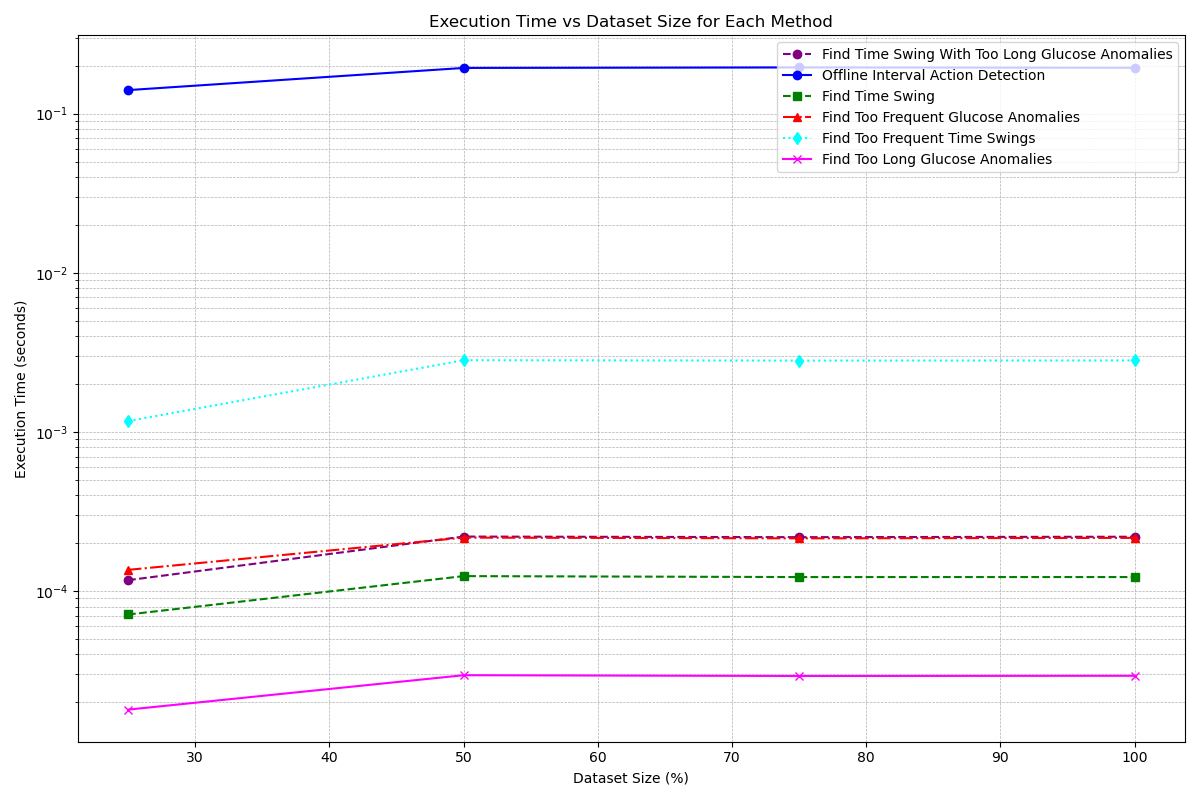
\includegraphics[width=01.0\textwidth]{Images/Graphs/execution_times.png}
\caption{Execution Times for Different Methods}
\label{fig:execution_times}
\end{figure}

\pagebreak

Figure \ref{fig:growth_rates} shows the average growth rates of execution times for each method as the dataset size increases.

\begin{figure}[h!]
\centering
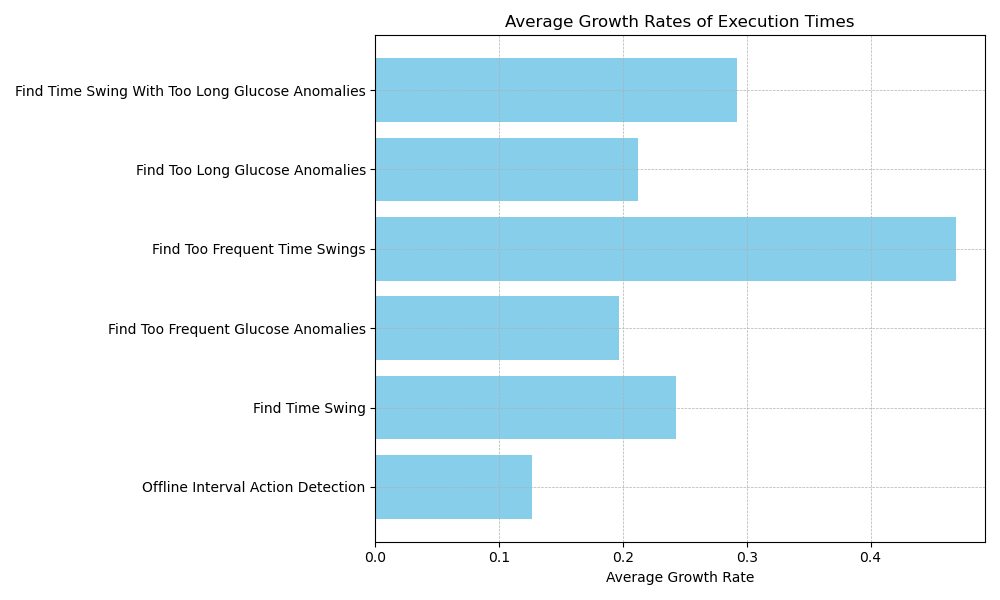
\includegraphics[width=01.0\textwidth]{Images/Graphs/growth_rates.png}
\caption{Average Growth Rates of Execution Times}
\label{fig:growth_rates}
\end{figure}

\subsubsection{Final Considerations}

\begin{itemize}
    \item \textbf{General Efficiency}: Most methods show very short execution times, typically in the millisecond range, with minimal impact from dataset size.
    \item \textbf{Scalability of the Main Method}: The \texttt{offline\_interval\_action\_detection} method exhibits moderate scalability with an average execution time of 0.1808 seconds and a growth rate of 0.1267.
    \item \textbf{Other Methods}: Methods like \texttt{find\_too\_long\_glucose\_anomalies} and \texttt{find\_too\_frequent\_glucose\_anomalies} show negligible growth with average execution times of 0.00002658 and 0.00019583 seconds, respectively.
    \item \textbf{Growth Trends}: Growth rates are higher for methods like \texttt{find\_too\_frequent
    \_time\_swings} and \texttt{find\_time\_swing\_with\_too\_long\_glucose\_anomalies}, but overall, execution times increase moderately with dataset size.
\end{itemize}

In summary, the system demonstrates good efficiency and acceptable scalability. The \texttt{offline\_interval\_action\_detection} method requires further optimization attention, while other methods handle increasing data sizes well.

\subsection{Conclusions and Future Work}

The analysis of glucose data using implemented functions and classes has provided precise insights into glucose level changes over time, identification of significant anomalies in the duration and frequency of glycemic events, and recognition of important Time Swings. These results are critical for enhancing diabetes management, enabling timely interventions, and customizing treatment based on specific data points.

Future work will focus on improving the analysis of high-level events identified in the current implementation and researching and studying additional significant events. Additionally, the website will address and remove existing limitations, such as the restriction of one CSV file per patient and the lack of graphical representations, to provide a more comprehensive data management and analysis tool.

Moreover, there are plans to develop a mobile version of the website. This will offer several advantages, including increased accessibility for users on-the-go, real-time data monitoring and updates, and a more user-friendly interface for managing patient records and analyzing glucose data.

By enhancing event analysis, removing current limitations, and creating a mobile version, the website will significantly improve its utility and effectiveness in diabetes management and patient care.

\pagebreak

\section*{References}

\begin{enumerate}

  \item \textbf{Flask}
    \begin{quote}
        Micro framework per Python. \url{https://flask.palletsprojects.com}
    \end{quote}
    
    \item \textbf{Laravel}
    \begin{quote}
        Framework PHP per lo sviluppo web. \url{https://laravel.com}
    \end{quote}

    \item \textbf{MySQL}
    \begin{quote}
        Database open-source. \url{https://www.mysql.com}
    \end{quote}

    \item \textbf{ISEQL}
    \begin{quote}
        F. Persia and S. Helmer, "A Framework for High-Level Event Detection in a Social Network Context Via an Extension of ISEQL," 2018 IEEE 12th International Conference on Semantic Computing (ICSC), Laguna Hills, CA, USA, 2018, pp. 140-147, doi: 10.1109/ICSC.2018.00028.
    \end{quote}
    
    \item \textbf{SOCO}
    \begin{quote}
        Project by Fabio Persia. Full project title: "Modeling and Detecting High-Level Events in Healthcare Applications Exploiting ISEQL+."
    \end{quote}
\end{enumerate}
    
\end{document}
